% !TEX program = LuaLaTeX+se
% !TEX encoding = UTF-8

\documentclass[12pt]{article} % use larger type; default would be 10pt

% usual packages loading:
\usepackage{forloop}
\usepackage{calc}
\usepackage{fontspec}
\usepackage{graphicx} % support the \includegraphics command and options
\usepackage[allowdeprecated=false]{gregoriotex} % for gregorio score inclusion
\usepackage{fullpage} % to reduce the margins
\usepackage{titlesec}
\usepackage[oldstyle]{libertine}
\usepackage{lettrine}
\setlength{\parindent}{-0.25in}
% for English psalm pointing
\usepackage[normalem]{ulem}
\setlength{\ULdepth}{2pt}

% Repeat something:
\newcounter{loopcntr}
\newcommand{\repeatthing}[2][1]{%
  \forloop{loopcntr}{0}{\value{loopcntr}<#1}{#2}%
}

% dual language parallel text thing
\usepackage{reledmac}
\usepackage{reledpar}

% STYLE FOR THE TITLE PAGE
\usepackage{fancyhdr}
\pagestyle{fancy}
\lhead{}
\chead{\color{benblue1}{ \repeatthing[17]{\greornamentation{2}{12}} }}
\rhead{}
\lfoot{}
\cfoot{\color{benblue1}{ \repeatthing[17]{\greornamentation{2}{12}} }\\ \color{black}\thepage}
\rfoot{}
\renewcommand{\headrulewidth}{0pt}
\setlength{\headsep}{25pt}

%the bilingual stuff seems to necessitate this stuff being reset each time;
%without this function the initial letter ends up much smaller and the red antiphon number
%appears over top of the initial, not above it as desired
\newcommand{\myaboveinitial}[1]{%
    \expandafter\renewcommand\csname greinitialformat\endcsname[1]{%
        \fontsize{43}{43}\selectfont ##1
    }
    \gresetfirstlineaboveinitial{\textcolor{benred8}{\raisebox{6.0mm}{\small \textsc{\textbf{#1}}}}}{}
}

% RED
\definecolor{benred8}{HTML}{E82C00} 

% BLUE
\definecolor{benblue1}{HTML}{2B22C7}

% YELLOWS
\definecolor{benyellow1}{HTML}{FFD435}
\definecolor{benyellow2}{HTML}{7C6F3B}

% DEFINE THE FORMATTING OF
% PSALM TEXT
\newenvironment{psalmtext}{\leftskip 0.25in}{\vspace{2 mm}}
\newenvironment{rubric}{\color{benred8} \itshape \leftskip 0in \setlength{\parindent}{0.25in}}{\vspace{2 mm}}
\newenvironment{response}{\leftskip 0in \setlength{\parindent}{0in}}{\vspace{2 mm}}
\newenvironment{lettrinePar}
  {\par\leftskip=0.30in \rightskip=0em}
  {\par} % since switching to reledpar from eledpar lettrine no longer seems to work properly!
         % this environment is a compromise

% REDUCES SUBSECTION SPACE
\def\subspace{\vspace{-13 mm}}

% MAKES Flexa : TEXT
\def\flex{\textit{\textcolor{benred8}{Flexa :}}}

% MAKES Flex : TEXT
\def\flexeng{\textit{\textcolor{benred8}{Flex :}}}

% MAKES Cantor : TEXT
\def\cantor{\textit{\textcolor{benred8}{Cantor :}}}

% MAKES vel : TEXT
\def\vel{\textit{\textcolor{benred8}{vel :}}}

% MAKES deinde : TEXT
\def\deinde{\textit{\textcolor{benred8}{deinde :}}}

% MAKES Repetitur : TEXT
\def\repetitur{\textit{\textcolor{benred8}{Repetitur :}}}

% MAKES Repeat: TEXT
\def\repetitureng{\textit{\textcolor{benred8}{Repeat:}}}

% MAKES secreto usque ad TEXT
\def\secreto{\textit{\textcolor{benred8}{secreto usque ad}}}

% MAKES secret until TEXT
\def\secretoeng{\textit{\textcolor{benred8}{secret until}}}

% MAKES T.P. TEXT
\def\TemporePaschale{\textit{\textcolor{benred8}{T. P.}}}

% MAKES RED PIPE FOR ENGLISH CADENCES
\def\pipe{\textcolor{benred8}{\symbol{"01C1}}}

% MAKES ALL \GreStars RED
\let\OldGreStar\GreStar
\renewcommand{\GreStar}{\textcolor{benred8}{\OldGreStar}}

% MAKES ALL \GreDaggers RED
\let\OldGreDagger\GreDagger
\renewcommand{\GreDagger}{\textcolor{benred8}{\OldGreDagger}}

% MAKES ALL \Vbars RED
\let\oldVbar\Vbar
\def\VVbar{\textcolor{benred8}{\oldVbar\oldVbar .}}
\renewcommand{\Vbar}{\textcolor{benred8}{\oldVbar .}}

% MAKES ALL \Rbars RED
\let\oldRbar\Rbar
\renewcommand{\Rbar}{\textcolor{benred8}{\oldRbar .}}

% MAKES ALL \Abars RED
\let\oldAbar\Abar
\renewcommand{\Abar}{\textcolor{benred8}{\oldAbar .}}

% MAKES ALL \grealtcrosses RED
\let\oldgrealtcross\grealtcross
\renewcommand{\grealtcross}{\textcolor{benred8}{\oldgrealtcross}}

% ANOTHER CROSS GLYPH USED FOR THE SIGN OF THE CROSS WITH THUMB ON CHEST
\newcommand{\grebencross}{\fontspec{gresym3.ttf}\textcolor{benred8}{T}}

% FORMAT SECTIONS - use titlesec package
\titleformat{\section}{\centering\scshape\Huge\color{benred8}}{}{1em}{}
\titlespacing*{\section}{0pt}{0pt}{0pt}

% FORMAT SUBSECTIONS - use titlesec package
\titleformat{\subsection}{\centering\normalfont\color{benred8}}{}{1em}{}
\titlespacing*{\subsection}{0pt}{0pt}{0.25pt}

% RED TITLE e.g Psalm number, "Oratio", "Capitulum", etc.
\newcommand{\redTitle}[1]{{
\centering
\textcolor{benred8}{#1}

}}


% SPACE BETWEEN Capitulum AND BIBLE VERSE
\def\capitulumSpace{\hspace{20 mm}}

% ANNOTATION STYLE
\grechangestyle{annotation}{\small\scshape\bfseries\color{benred8}}
\grechangedim{annotationraise}{-3 mm}{scalable}

% Sicut incensum R/ indent, e.g. versicle after first hymn at Sunday Vespers
\newlength{\sicutIncensumIndent}
\setlength{\sicutIncensumIndent}{2.3mm}


%%%%%%%%%%%%%%%%%%%%%%%%%%%%
% HERE BEGINS THE DOCUMENT %
%%%%%%%%%%%%%%%%%%%%%%%%%%%%

\begin{document}

\pagenumbering{gobble}

\begin{center}

\color{benred8}

{\fontsize{2.660cm}{5 em}\selectfont

PSALTERIUM

}

\vspace*{15 pt}

{\fontsize{2.975cm}{5 em}\selectfont

VESPERALE

}

\vspace*{20 pt}

{\fontsize{1.5cm}{1 em}\selectfont

JUXTA RITUM

\vspace*{2.7 mm}

ROMANUM

\vspace*{5 mm}

ANTIQUIOREM

}

\vspace*{5 mm}

\begin{Huge}

ANNOTATUM

\end{Huge}\begin{Large}

AC

\vspace*{-1.0 mm}

\end{Large}\begin{Huge}

SIGNIS RHYTHMICIS ORNATUM

\end{Huge}

\vspace*{8 mm}

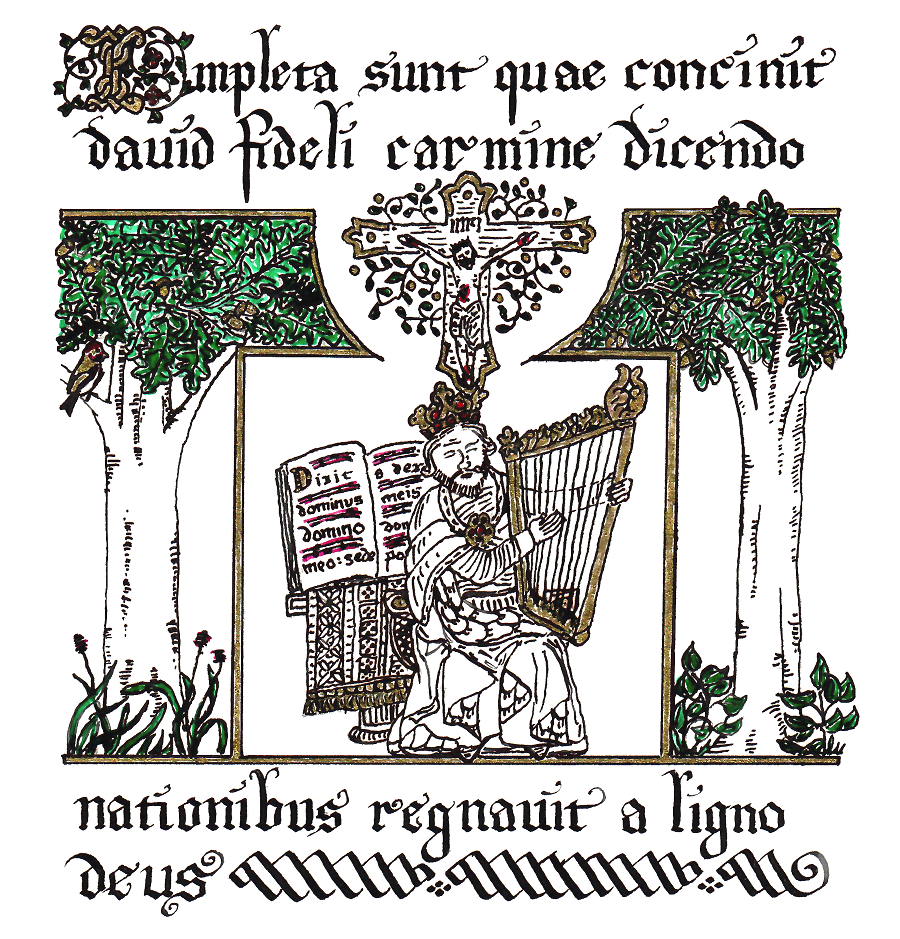
\includegraphics[height=7.20cm]{David2017s.png}

\vspace*{6 mm}

\begin{large}

\textsc{a.d. mmxvii}

\end{large}

\end{center}

%redefine 'plain' page style to have blue page numbers too
\fancypagestyle{plain}{
	\chead{}
	\cfoot{\textcolor{benblue1}{\thepage}}

}

\newpage
\thispagestyle{empty}
\mbox{}
\newpage
\thispagestyle{empty}
\mbox{}
\newpage

\chead{\color{benred8}\textsc{Dominica \textemdash\ Sunday}}
\cfoot{\textcolor{benblue1}{\thepage}}
\thispagestyle{plain}
\pagenumbering{arabic}
\setcounter{page}{4}

%%%%%%%%%%%%%%%%%%%%%%%%%%%%%%%%%%%%%%%%%%%%%%%%%%%%%%
%%%%%%%%%%%%%%%%%%%%%%%%%%%%%%%%%%%%%%%%%%%%%%%%%%%%%%

% SUNDAY VESPERS
% DOMINICA AD VESPERAS
% START PARALLEL TEXTS
\begin{pages}
\begin{Leftside}
\firstlinenum{10000}\linenumincrement{10000}\beginnumbering\pstart

\begin{center}\begin{Huge}\textsc{\textcolor{benred8}{Dominica ad Vesperas}}\end{Huge}\end{center}

\pend\pstart

\vspace{2mm}

\begin{center}Pater no\libertineGlyph{s_t}er. Ave Mar\'{i}a.\end{center}

\pend\pstart

\grechangestyle{initial}{\fontsize{43}{43}\selectfont}
\greannotation{\upshape\Vbar}
\gregorioscore[a]{LatinVersion/DeusInAdjutorium.gtex}

\pend\pstart

\begin{rubric}
A Septuagesima usque ad Pascha, loco \emph{\textcolor{black}{Allelúia}}, canitur :

\end{rubric}

\gregorioscore[a]{LatinVersion/LausTibi.gtex}

\pend\pstart

\vspace{2mm}

\begin{center}\begin{large}\textbf{\textsc{\textcolor{benred8}{1 Antiphona. VII c 2}}}\end{large}\end{center}

\vspace{2mm}

\pend\pstart

{\gresetinitiallines{2}
\grechangestyle{initial}{\fontsize{160}{160}\selectfont}
\gregorioscore[a]{LatinVersion/Dominica/DomAnt1-01.gtex}

}

\pend\pstart

\redTitle{Psalmus 109.}

\pend\pstart

\begin{psalmtext}
% Donec ponam ini\textbf{mí}cos \textbf{tu}os, \GreStar\ scabéllum \textbf{pe}dum tu\textbf{ó}rum.

Virgam virtútis tuæ emíttet Dómi\textbf{nus} ex \textbf{Si}on : \GreStar\ domináre in médio inimi\textbf{có}rum tu\textbf{ó}rum.

Tecum princípium in die virtútis tuæ in splendóri\textbf{bus} sanc\textbf{tó}rum : \GreStar\ ex útero ante lucíferum \textbf{gé}nu\textbf{i} te.

Jurávit Dóminus et non pæni\textbf{té}bit \textbf{e}um : \GreStar\ Tu es sacérdos in æt\'{e}rnum secúndum órdi\textbf{nem} Mel\textbf{chí}sedech.

Dóminus a \textbf{dex}tris \textbf{tu}is, \GreStar\ confrégit in die iræ \textbf{su}æ \textbf{re}ges.

Judicábit in natiónibus, im\textbf{plé}bit ru\textbf{í}nas : \GreStar\ conquassábit cápita in \textbf{ter}ra mul\textbf{tó}rum.

De torrénte in \textbf{vi}a \textbf{bi}bet : \GreStar\ proptérea exal\textbf{tá}bit \textbf{ca}put.

Glória \textbf{Pa}tri, et \textbf{Fí}lio, \GreStar\ et Spi\textbf{rí}tui \textbf{Sanc}to.

Sicut erat in princípio, et \textbf{nunc}, et \textbf{sem}per, \GreStar\ et in sǽcula sæcu\textbf{ló}rum. \textbf{A}men.

\end{psalmtext}

\pend\pstart

\gregorioscore[a]{LatinVersion/Dominica/DomAnt1-02.gtex}

\pend\pstart

%% DOMINICA 2 ANT.

\greannotation{2 {\upshape\Abar} IV g}
\gregorioscore[a]{LatinVersion/Dominica/DomAnt2-01.gtex}

\pend\pstart

\redTitle{Psalmus 110.}

\pend\pstart

\gregorioscore[a]{LatinVersion/Dominica/DomFL2.gtex}

\pend\pstart

\begin{psalmtext}
Magna ó\emph{pera} \textbf{Dó}mini : \GreStar\ exquisíta in omnes voluntátes \textbf{e}jus.

Conféssio et magnificéntia \emph{opus} \textbf{e}jus : \GreStar\ et ju\libertineGlyph{s_t}ítia ejus manet in sǽculum \textbf{sǽ}culi.

Memóriam fécit mirabílium suórum, \GreDagger\ miséricors et mise\emph{rátor} \textbf{Dó}minus : \GreStar\ escam dedit timénti\textbf{bus} se.

Memor erit in sǽculum te\libertineGlyph{s_t}a\emph{ménti} \textbf{su}i : \GreStar\ virtútem óperum suórum annuntiábit pópulo \textbf{su}o :

Ut det illis hæredi\emph{tátem} \textbf{gén}tium : \GreStar\ ópera mánuum ejus véritas et ju\textbf{dí}cium.

Fidélia ómnia mandáta ejus : \GreDagger\ confirmáta in sǽ\emph{culum} \textbf{sǽ}culi : \GreStar\ fa\libertineGlyph{c_t}a in veritáte et æqui\textbf{tá}te.

Redemptiónem misit pó\emph{pulo} \textbf{su}o : \GreStar\ mandávit in ætérnum te\libertineGlyph{s_t}améntum \textbf{su}um.

\textcolor{benred8}{\emph{Fit reverentia :}} San\libertineGlyph{c_t}um et terríbile \emph{nomen} \textbf{e}jus : \GreStar\ inítium sapiéntiae timor \textbf{Dó}mini.

Intellé\libertineGlyph{c_t}us bonus ómnibus facién\emph{tibus} \textbf{e}um : \GreStar\ laudátio ejus manet in sǽculum \textbf{sǽ}culi.

Glória Pa\emph{tri, et} \textbf{Fí}lio, \GreStar\ et Spirítui \textbf{Sanc}to.

Sicut erat in princípio, et \emph{nunc, et} \textbf{sem}per, \GreStar\ et in sǽcula sæculórum. \textbf{A}men.

\end{psalmtext}

\pend\pstart

\gregorioscore[a]{LatinVersion/Dominica/DomAnt2-02.gtex}

\pend\pstart

%% DOMINICA 3 ANT.

\greannotation{3 {\upshape\Abar} IV a}
\gregorioscore[a]{LatinVersion/Dominica/DomAnt3-01.gtex}

\pend\pstart

\redTitle{Psalmus 111.}

\pend\pstart

\gregorioscore[a]{LatinVersion/Dominica/DomFL3.gtex}

\pend\pstart

\begin{psalmtext}
Potens in terra erit \emph{semen} \textbf{e}jus : \GreStar\ generátio re\libertineGlyph{c_t}órum \emph{benedi}\textbf{cé}tur.

Glória et divítiae in \emph{domo} \textbf{e}jus : \GreStar\ et ju\libertineGlyph{s_t}ítia ejus manet in \emph{sǽculum} \textbf{sǽ}culi.

Exórtum e\libertineGlyph{s_t} in ténebris \emph{lumen} \textbf{rec}tis : \GreStar\ miséricors, et mise\emph{rátor, et} \textbf{jus}tus.

Jucúndus homo qui miserétur et cómmodat, \GreDagger\ dispónet sermónes suos \emph{in ju}\textbf{dí}cio : \GreStar\ quia in ætérnum \emph{non commo}\textbf{vé}bitur.

In memória ætérna \emph{erit} \textbf{jus}tus : \GreStar\ ab auditióne ma\emph{la non ti}\textbf{mé}bit.

Parátum cor ejus speráre in Dómino, \GreDagger\ confirmátum \emph{e\libertineGlyph{s_t} cor} \textbf{e}jus : \GreStar\ non commovébitur donec despíciat i\emph{nimícos} \textbf{su}os.

Dispérsit, dedit paupéribus : \GreDagger\ ju\libertineGlyph{s_t}ítia ejus manet in sǽ\emph{culum} \textbf{sǽ}culi : \GreStar\ cornu ejus exaltá\emph{bitur in} \textbf{gló}ria.

Peccátor vidébit, et irascétur, \GreDagger\ déntibus suis fremet \emph{et ta}\textbf{bé}scet : \GreStar\ desidérium pecca\emph{tórum pe}\textbf{rí}bit.

Glória Pa\emph{tri, et} \textbf{Fí}lio, \GreStar\ et Sp\emph{irítui} \textbf{Sanc}to.

Sicut erat in princípio, et \emph{nunc, et} \textbf{sem}per, \GreStar\ et in sǽcula sæ\emph{culórum}. \textbf{A}men.

\end{psalmtext}

\pend\pstart

\gregorioscore[a]{LatinVersion/Dominica/DomAnt3-02.gtex}

\pend\pstart

%% DOMINICA 4 ANT.

\vspace{2mm}

\greannotation{4 {\upshape\Abar} VII c}
\gregorioscore[a]{LatinVersion/Dominica/DomAnt4-01.gtex}

\pend\pstart

\redTitle{Psalmus 112.}

\pend\pstart

\gregorioscore[a]{LatinVersion/Dominica/DomFL4.gtex}

\pend\pstart

\begin{psalmtext}
\textcolor{benred8}{\emph{Fit reverentia :}} Sit nomen Dómini \textbf{be}ne\textbf{díc}tum, \GreStar\ ex hoc nunc, et \textbf{us}que in \textbf{sǽ}culum.

A solis ortu usque \textbf{ad} oc\textbf{cá}sum, \GreStar\ laudábile \textbf{no}men \textbf{Dó}mini.

Excélsus super omnes \textbf{gen}tes \textbf{Dó}minus, \GreStar\ et super cælos \textbf{gló}ria \textbf{e}jus.

Quis sicut Dóminus Deus no\libertineGlyph{s_t}er, qui in \textbf{al}tis \textbf{há}bitat, \GreStar\ et humília réspicit in cælo \textbf{et} in \textbf{ter}ra?

Súscitans a \textbf{ter}ra \textbf{í}nopem, \GreStar\ et de \libertineGlyph{s_t}ércore \textbf{é}rigens \textbf{páu}perem :

Ut cóllocet eum \textbf{cum} prin\textbf{cí}pibus, \GreStar\ cum princípibus \textbf{pó}puli \textbf{su}i.

Qui habitáre facit \libertineGlyph{s_t}éri\textbf{lem} in \textbf{do}mo, \GreStar\ matrem fili\textbf{ó}rum lae\textbf{tán}tem.

Glória \textbf{Pa}tri, et \textbf{Fí}lio, \GreStar\ et Spi\textbf{rí}tui \textbf{Sanc}to.

Sicut erat in princípio, et \textbf{nunc}, et \textbf{sem}per, \GreStar\ et in sǽcula sæcu\textbf{ló}rum. \textbf{A}men.

\end{psalmtext}

\pend\pstart

\gregorioscore[a]{LatinVersion/Dominica/DomAnt4-02.gtex}

\pend\pstart

%% DOMINICA 5 ANT.

\greannotation{5 {\upshape\Abar} T. Per.}
\gregorioscore[a]{LatinVersion/Dominica/DomAnt5-01.gtex}

\pend\pstart

\redTitle{Psalmus 113.}

\pend\pstart

\gregorioscore[a]{LatinVersion/Dominica/DomFL5.gtex}

\pend\pstart

\begin{psalmtext}
Fa\libertineGlyph{c_t}a e\libertineGlyph{s_t} Judǽa san\libertineGlyph{c_t}ifi\emph{cátio} \textbf{e}jus, \GreStar\ Israel potés\emph{tas} \textbf{e}jus.

Mare \emph{vidit, et} \textbf{fu}git : \GreStar\ Jordánis convérsus e\libertineGlyph{s_t} \emph{re}\textbf{trór}sum.

Montes exsultavé\emph{runt ut a}\textbf{rí}etes : \GreStar\ et colles sicut a\emph{gni} \textbf{ó}vium.

Quid e\libertineGlyph{s_t} tibi ma\emph{re quod fu}\textbf{gís}ti? \GreStar\ et tu Jordánis, quia convérsus es \emph{re}\textbf{trór}sum.

Montes exsultá\libertineGlyph{s_t}is \emph{sicut a}\textbf{rí}etes, \GreStar\ et colles sicut a\emph{gni} \textbf{ó}vium?

A fácie Dómini \emph{mota e\libertineGlyph{s_t}} \textbf{ter}ra, \GreStar\ a fácie De\emph{i} \textbf{Ja}cob : 

Qui convértit petram in \emph{\libertineGlyph{s_t}agna a}\textbf{quá}rum, \GreStar\ et rupem in fontes \emph{a}\textbf{quá}rum.

Non nobis Dó\emph{mine, non} \textbf{no}bis : \GreStar\ sed nómini tuo \emph{da} \textbf{gló}riam.

Super misericórdia tua et ve\emph{ritáte} \textbf{tu}a : \GreStar\ nequándo dicant gentes : Ubi e\libertineGlyph{s_t} Deus \emph{e}\textbf{ó}rum?

Deus autem \emph{no\libertineGlyph{s_t}er in} \textbf{cæ}lo : \GreStar\ ómnia quæcúmque vólu\emph{it}, \textbf{fe}cit.

Simulácra géntium ar\emph{géntum et} \textbf{au}rum, \GreStar\ ópera mánu\emph{um} \textbf{hó}minum.

Os habent, \emph{et non lo}\textbf{quén}tur : \GreStar\ óculos habent, et non \emph{vi}\textbf{dé}bunt.

Aures ha\emph{bent, et non} \textbf{áu}dient : \GreStar\ nares habent, et non o\emph{do}\textbf{rá}bunt.

Manus habent, et non palpábunt : \GreDagger\ pedes habent, et \emph{non ambu}\textbf{lá}bunt : \GreStar\ non clamábunt in gúttu\emph{re} \textbf{su}o.

Símiles illis fiant qui \emph{fáciunt} \textbf{e}a : \GreStar\ et omnes qui confídunt \emph{in} \textbf{e}is.

Domus Israel spe\emph{rávit in} \textbf{Dó}mino : \GreStar\ adjútor eórum et proté\libertineGlyph{c_t}or \emph{e}\textbf{ó}rum e\libertineGlyph{s_t}.

Domus Aaron spe\emph{rávit in} \textbf{Dó}mino : \GreStar\ adjútor eórum et proté\libertineGlyph{c_t}or \emph{e}\textbf{ó}rum e\libertineGlyph{s_t}.

Qui timent Dóminum spera\emph{vérunt in} \textbf{Dó}mino : \GreStar\ adjútor eórum et proté\libertineGlyph{c_t}or \emph{e}\textbf{ó}rum e\libertineGlyph{s_t}.

Dóminus me\emph{mor fuit} \textbf{nos}tri : \GreStar\ et benedí\emph{xit} \textbf{no}bis.

Benedíxit \emph{dómui} \textbf{Is}rael : \GreStar\ benedíxit dómu\emph{i} \textbf{A}aron.

Benedíxit ómnibus \emph{qui timent} \textbf{Dó}minum \GreStar\ pusíllis cum \emph{ma}\textbf{jór}ibus.

Adjíciat \emph{Dóminus} \textbf{su}per vos : \GreStar\ super vos, et super fíli\emph{os} \textbf{ves}tros.

Benedíc\emph{ti vos a} \textbf{Dó}mino, \GreStar\ qui fecit cælum \emph{et} \textbf{ter}ram.

Cæ\emph{lum cæli} \textbf{Dó}mino : \GreStar\ terram autem dedit fíli\emph{is} \textbf{hó}minum.

Non mórtui lau\emph{dábunt te} \textbf{Dó}mine : \GreStar\ neque omnes qui descéndunt in \emph{in}\textbf{fér}num.

Sed nos qui vívimus bene\emph{dícimus} \textbf{Dó}mino, \GreStar\ ex hoc nunc et usque \emph{in} \textbf{sǽ}culum.

Glória \emph{Patri, et} \textbf{Fí}lio, \GreStar\ et Spirítu\emph{i} \textbf{Sanc}to.

Sicut erat in princípio, \emph{et nunc, et} \textbf{sem}per, \GreStar\ et in sǽcula sæculó\emph{rum}. \textbf{A}men.

\end{psalmtext}

\pend\pstart

\gregorioscore[a]{LatinVersion/Dominica/DomAnt5-02.gtex}

\pend\pstart

\begin{rubric}
Sequens Capitulum \emph{\textcolor{black}{Bened\'{i}\libertineGlyph{c_t}us Deus}} canitur a Dominica II po\libertineGlyph{s_t}  Epiphaniam usque ad Septuagesimam, et a Dominica III po\libertineGlyph{s_t} Penteco\libertineGlyph{s_t}en usque ad Adventum tantum. Hymnus vero canitur in iisdem Dominicis po\libertineGlyph{s_t} Penteco\libertineGlyph{s_t}en et Epiphaniam, etiam usque ad Dominicam I Quadragesim\ae .

\end{rubric}

\pend\pstart

% DOMINICA CAPITULUM

\redTitle{Capitulum.\capitulumSpace \emph{2 Cor. 1, 3--4.}}

\label{DominicaCapitulum}

\pend\pstart

\vspace{-5mm}

\gregorioscore[a]{LatinVersion/CapitulumBenedictus.gtex}

\color{black}

\pend\pstart

% DOMINICA HYMNUS HIEME

\vspace{4mm}

\redTitle{Hymnus.\\Tonus in Hieme.}

\pend\pstart

\begin{rubric}
Sequens tonus canitur in Dominicis po\libertineGlyph{s_t} Epiphaniam a die 14 Januarii usque ad Dominicam Quinquagesim\ae\ inclusive, et a Dominica proximiori Kalendis O\libertineGlyph{c_t}obris scilicet a die 28 Septembris usque ad Dominicam ultimam po\libertineGlyph{s_t} Penteco\libertineGlyph{s_t}en.

\end{rubric}

\pend\pstart

\greannotation{IV}
\gregorioscore[a]{LatinVersion/Dominica/DomHym-Hieme.gtex}

\pend\pstart

\begin{rubric}
Quando fit Commemoratio B. M. V., canitur doxologia \emph{\textcolor{black}{Gl\'{o}ria tibi, D\'{o}mine, Qui natus es de V\'{i}rgine, Cum Patre \emph{et} Sancto Sp\'{i}ritu, In sempit\'{e}rna s\'{\ae}cula}}, sed non mutatur tonus hymni.

\end{rubric}

\pend\pstart

{\gresetinitiallines{0}
\gregorioscore[a]{LatinVersion/DirigaturDomine.gtex}

}

\begin{response}
\hspace{\sicutIncensumIndent}\Rbar\ Sicut \hspace{1.1mm} inc\'{e}nsum \hspace{1.1mm} in \hspace{1.1mm} consp\'{e}\libertineGlyph{c_t}u \hspace{1.2mm} tu- o.

\end{response}

\pend\pstart

% DOMINICA HYMNUS AESTATE

\redTitle{Tonus in \AE \libertineGlyph{s_t}ate.}

\pend\pstart

\begin{rubric}
Sequens tonus canitur in Dominica IV et reliquis Dominicis po\libertineGlyph{s_t} Penteco\libertineGlyph{s_t}en usque ad Dominicam proximiorem Kalendis O\libertineGlyph{c_t}obris id e\libertineGlyph{s_t} ad diem 27 Septembris inclusive occurrentibus.

\end{rubric}

\pend\pstart

\greannotation{VIII}
\gregorioscore[a]{LatinVersion/Dominica/DomHym-Aestate.gtex}

\pend\pstart

\begin{response}
\Vbar\ Dirig\'{a}tur D\'{o}mine or\'{a}tio mea.\\
\Rbar\ Sicut inc\'{e}nsum in consp\'{e}\libertineGlyph{c_t}u tuo.

\end{response}

\pend\pstart

% DOMINICA HYMNUS AD LIB 1

\redTitle{Tonus ad libitum I.}

\pend\pstart

\greannotation{VIII}
\gregorioscore[a]{LatinVersion/Dominica/DomHym-AdLib1.gtex}

\pend\pstart

\begin{response}
\Vbar\ Dirig\'{a}tur D\'{o}mine or\'{a}tio mea.\\
\Rbar\ Sicut inc\'{e}nsum in consp\'{e}\libertineGlyph{c_t}u tuo.

\end{response}

\pend\pstart

% DOMINICA HYMNUS AD LIB 2

\redTitle{Tonus ad libitum II.}

\pend\pstart

\greannotation{I}
\gregorioscore[a]{LatinVersion/Dominica/DomHym-AdLib2.gtex}

\pend\pstart

\begin{response}
\Vbar\ Dirig\'{a}tur D\'{o}mine or\'{a}tio mea.\\
\Rbar\ Sicut inc\'{e}nsum in consp\'{e}\libertineGlyph{c_t}u tuo.

\end{response}

\pend\pstart

% DOMINICA MAGNIFICAT

\vspace{1mm}

\redTitle{Canticum Beat\ae\ Mari\ae\ Virginis.\capitulumSpace \emph{Luc. 1, 46--55.}}

\pend\pstart

\begin{rubric}
Canitur Antiphona propria.

\end{rubric}

\pend\pstart

\vspace{-2mm}

\begin{psalmtext}
\lettrine[lhang=0.70]{M}{a}gn\'{i}ficat \grealtcross\ \'{a}nima mea D\'{o}minum :
%Magn\'{i}ficat \GreStar\ \'{a}nima mea D\'{o}minum :

\hspace*{9.5 mm}Et exsult\'{a}vit sp\'{i}ritus meus \GreStar\ in Deo salut\'{a}ri meo.

Quia resp\'{e}xit humilit\'{a}tem anc\'{i}ll\ae\ su\ae\ : \GreStar\ ecce enim ex hoc be\'{a}tam me dicent omnes generati\'{o}nes.

Quia fecit mihi magna qui potens e\libertineGlyph{s_t} : \GreStar\ et san\libertineGlyph{c_t}um nomen ejus.

Et miseric\'{o}rdia ejus a prog\'{e}nie in prog\'{e}nies \GreStar\ tim\'{e}ntibus eum.

Fecit pot\'{e}ntiam in br\'{a}chio suo : \GreStar\ disp\'{e}rsit sup\'{e}rbos mente cordis sui.

Dep\'{o}suit pot\'{e}ntes de sede, \GreStar\ et exalt\'{a}vit h\'{u}miles.

Esuri\'{e}ntes impl\'{e}vit bonis : \GreStar\ et d\'{i}vites dim\'{i}sit in\'{a}nes.

Susc\'{e}pit Israel p\'{u}erum suum, \GreStar\ record\'{a}tus miseric\'{o}rdi\ae\ su\ae.

Sicut loc\'{u}tus e\libertineGlyph{s_t} ad patres nostros, \GreStar\ Abraham, et s\'{e}mini ejus in s\'{\ae}cula.

Glória Patri, et Fílio, \GreStar\ et Spirítui San\libertineGlyph{c_t}o.

Sicut erat in princípio, et nunc, et semper, \GreStar\ et in sǽcula sæculórum. Amen.

\end{psalmtext}

\pend\pstart

\begin{rubric}
Deinde repetitur Antiphona.

\end{rubric}

\pend\pstart

\vspace{-5mm}

\redTitle{Oratio.}

\pend\pstart

\vspace{1mm}

{
\grechangedim{beforeinitialshift}{0.25mm}{scalable}
\grechangedim{afterinitialshift}{0.25mm}{scalable}
\greannotation{\upshape\Vbar}
\gregorioscore[a]{LatinVersion/DomineExaudi-short-01.gtex}

}

\pend\pstart

\begin{rubric}
Canitur Oratio propria, secundum tonum ut habetur in p.~\pageref{sec:TonusOrationis}, et post eam, si occurrat eo die aliquod Fe\libertineGlyph{s_t}um Simplex, vel ad modum Simplicis recolendum, fit de eo commemoratio. Po\libertineGlyph{s_t}remo (~si id tempus requirit~) fiunt Commemorationes de San\libertineGlyph{c_t}a Maria, de San\libertineGlyph{c_t}o Joseph, de Apo\libertineGlyph{s_t}olis, et de Patrono Ecclesi\ae\ in ordine aliarum Commemorationum secundum illius dignitatem, et ultimo loco de Pace, ut infra in p.~\pageref{sec:Commem}. Post ultimam Orationem canitur :

\end{rubric}

\pend\pstart

{
\grechangedim{beforeinitialshift}{0.25mm}{scalable}
\grechangedim{afterinitialshift}{0.25mm}{scalable}
\greannotation{\upshape\Vbar}
\gregorioscore[a]{LatinVersion/DomineExaudi-short-01.gtex}

}

\pend\pstart

\vspace{1mm}

\begin{rubric}
Per annum :

\end{rubric}

\pend\pstart

\vspace{-3mm}

\greannotation{I}
\gregorioscore[a]{LatinVersion/Dominica/DomBenedicamus.gtex}

\pend\pstart

\begin{rubric}
Tempore Adventus et Quadragesim\ae\ :

\end{rubric}

\pend\pstart

\greannotation{IV}
\gregorioscore[a]{LatinVersion/Dominica/DomBenedicamusAdvLent.gtex}

\pend\pstart

\greannotation{\upshape\Vbar}
\gregorioscore[a]{LatinVersion/FideliumAnimae.gtex}

\pend\pstart

\begin{rubric}
Si po\libertineGlyph{s_t} Vesperas immediate sequatur Completorium, di\libertineGlyph{c_t}o \Vbar\ \emph{\textcolor{black}{Fid\'{e}lium \'{a}nim\ae}}, \libertineGlyph{s_t}atim incipitur \Vbar\ \emph{\textcolor{black}{Jube D\'{o}mine bened\'{i}cere}}. Secus autem, si tunc terminetur Officium, dicitur \emph{\textcolor{black}{Pater no\libertineGlyph{s_t}er}} totum secreto. %Oratione Dominica secreto recitata, dicitur : %, ut infra ad Completorium.

\end{rubric}

\pend\endnumbering
\end{Leftside}
%%%%%%%%%%%%%%%%%%%%%%%%%%%%%%%%%%%%%%%%%%%%%%%%%%%%%%
%%%%%%%%%%%%%%%%%%%%%%%%%%%%%%%%%%%%%%%%%%%%%%%%%%%%%%
\begin{Rightside}

\firstlinenum{10000}\linenumincrement{10000}\beginnumbering\pstart

% SUNDAY AT VESPERS

\begin{center}\begin{Huge}\textsc{\textcolor{benred8}{Sunday at Vespers}}\end{Huge}\end{center}

\pend\pstart

\vspace{2mm}

\begin{center}Our Father. Hail Mary.\end{center}

\pend\pstart

\grechangestyle{initial}{\fontsize{43}{43}\selectfont}
\greannotation{\upshape\Vbar}
\gregorioscore[a]{EnglishVersion/DeusInAdjutorium.gtex}

\pend\pstart

\begin{rubric}
The following is sung from Septuagesima Sunday until Easter in place of \emph{\textcolor{black}{Alleluia}} :

\end{rubric}

\gregorioscore[a]{EnglishVersion/LausTibi.gtex}

\pend\pstart

\vspace{2mm}

\begin{center}\begin{large}\textbf{\textsc{\textcolor{benred8}{1 Antiphon. VII c 2}}}\end{large}\end{center}

\vspace{2mm}

\pend\pstart

{\gresetinitiallines{2}
\grechangestyle{initial}{\fontsize{160}{160}\selectfont}
\gregorioscore[a]{EnglishVersion/Dominica/DomAnt1-01.gtex}

}

\pend\pstart

\redTitle{Psalm 109.}

\pend\pstart

\begin{psalmtext}
%The Lord \textbf{said} to \textbf{my} Lord: \GreStar\ Sit thou \textbf{at} my \textbf{right} hand:

%Until I \textbf{make} thy \textbf{e}nemies \GreStar\ thy \textbf{foot}stool.

The Lord will send forth the sceptre of thy power \pipe\ out of Sion: \GreStar\ rule thou in the \pipe\ midst \uline{of~thy}\hspace{2mm}\uline{ene}mies.

With thee is the principality in the day of thy strength: in the \pipe\ brightness \uline{of the} saints: \GreStar\ from the womb before the day star \pipe\ I begot thee.

The Lord hath sworn, and \pipe\ he will \uline{not re}pent: \GreStar\ Thou art a priest for ever according to the order \pipe\ of Mel\uline{chise}dech.

The Lord \pipe\ at thy right hand \GreStar\ hath broken kings in the \pipe\ \textbf{day} \uline{of his} wrath.

He shall judge among nations, \pipe\ he \uline{shall fill} ruins: \GreStar\ he shall crush the heads in the \pipe\ land of many.

He shall drink of the \pipe\ torrent \uline{in the} way: \GreStar\ therefore shall he \pipe\ \textbf{lift} \uline{up the} head.

Glory be to the \pipe\ Fa\uline{ther, and}\hspace{2mm}\uline{to the} Son, \GreStar\ and to the \pipe\ Holy Spirit.

As it was in the beginning, is now, and \pipe\ ever shall be, \GreStar\ world without \pipe\ \textbf{end}. Amen.

\end{psalmtext}

\pend\pstart

\gregorioscore[a]{EnglishVersion/Dominica/DomAnt1-02.gtex}

\pend\pstart

%% SUNDAY 2 ANT.

\greannotation{2 {\upshape\Abar} IV g}
\gregorioscore[a]{EnglishVersion/Dominica/DomAnt2-01.gtex}

\pend\pstart

\redTitle{Psalm 110.}

\pend\pstart

\gregorioscore[a]{EnglishVersion/Dominica/DomFL2.gtex}

\pend\pstart

\begin{psalmtext}
%I will praise thee, O Lord, \emph{with my} \textbf{whole} heart ; \GreStar\ in the council of the just, and in the congre\textbf{ga}tion.

Great are \pipe\ the \textbf{works} \uline{of the} Lord: \GreStar\ sought out according to all \pipe\ his wills.

His work is \pipe\ praise and magni\uline{ficence}: \GreStar\ and his justice continueth for ever and \pipe\ ever.

He hath made a remembrance of his wonderful works, \GreDagger\ being a mer- \pipe\ ciful and gra\uline{cious~Lord}:~\GreStar\ he hath given food to them that \pipe\ fear him.

He will be mindful for e- \pipe\ ver of his co\uline{venant}: \GreStar\ he will shew forth to his people the power of \pipe\ his works.

That he may give them the inheri- \pipe\ tance of the Gentiles: \GreStar\ the works of his hands are truth and \pipe\ judgment.

All his commandments are faithful: \GreDagger\ confirmed for \pipe\ ever and ever, \GreStar\ made in truth and \pipe\ e\uline{quity}.

He hath sent redemp- \pipe\ tion to his people: \GreStar\ he hath commanded his covenant for \pipe\ ever.

\textcolor{benred8}{\emph{A sign of reverence is made:}} Holy and terri- \pipe\ ble \textbf{is} his name : \GreStar\ the fear of the Lord is the beginning of \pipe\ wisdom.

A good understanding \pipe\ to all that do it: \GreStar\ his praise continueth for ever and \pipe\ ever.

Glory be to the Father, \pipe\ and \textbf{to} the Son, \GreStar\ and to the Holy \pipe\ Spirit.

As it was in the beginning, is now, \pipe\ and ever shall be, \GreStar\ world without end. \pipe\ Amen.

\end{psalmtext}

\pend\pstart

\gregorioscore[a]{EnglishVersion/Dominica/DomAnt2-02.gtex}

\pend\pstart

 %% SUNDAY 3 ANT.

\greannotation{3 {\upshape\Abar} IV a}
\gregorioscore[a]{EnglishVersion/Dominica/DomAnt3-01.gtex}

\pend\pstart

\redTitle{Psalm 111.}

\pend\pstart

\gregorioscore[a]{EnglishVersion/Dominica/DomFL3.gtex}


\pend\pstart

\begin{psalmtext}
%Blessed is the man that \emph{feareth} \textbf{the} Lord: \GreStar\ he shall delight exceedingly \emph{in his com}\textbf{mand}ments.

His seed shall be \pipe\ migh\uline{ty up}\textbf{on} earth: \GreStar\ the generation of the right- \pipe\ eous \textbf{shall} be \uline{blessed}.

Glory and wealth shall \pipe\ be \textbf{in} his house: \GreStar\ and his justice remaineth for \pipe\ \textbf{e}ver and \uline{ever}.

To the righteous a light is \pipe\ risen up in \uline{darkness}: \GreStar\ he is merciful, and com- \pipe\ passionate and just.

Acceptable is the man that sheweth mercy and lendeth: \GreDagger\ he shall or- \pipe\ der his words with \uline{judgment}: \GreStar\ because he shall not \pipe\ be \textbf{moved} for \uline{ever}.

The just shall be in ever- \pipe\ \textbf{last}ing re\underline{membrance}: \GreStar\ he shall not fear \pipe\ the \textbf{e}vil \uline{hearing}.

His heart is ready to hope in the Lord: \GreDagger\ \pipe\ his \textbf{heart} is \uline{strengthened}, \GreStar\ he shall not be moved until he look \pipe\ over his e\uline{nemies}.

He hath distributed, he hath given to the poor: \GreDagger\ his justice remaineth \pipe\ for ever and \uline{ever}: \GreStar\ his horn shall be ex- \pipe\ \textbf{al}ted in \uline{glory}.

The wicked shall see, and shall be angry, \GreDagger\ he shall gnash with his \pipe\ \uline{\textbf{teeth} and}\hspace{2mm}\uline{\textbf{pine} a}way: \GreStar\ the desire of the \pipe\ \textbf{wi}cked shall \uline{perish}.

Glory be to the Father, \pipe\ and \textbf{to} the Son, \GreStar\ and to the \pipe\ \textbf{Holy} \uline{Spirit}.

As it was in the beginning, is now, \pipe\ and ever shall be, \GreStar\ world \pipe\ \uline{without} \textbf{end}. Amen.

\end{psalmtext}

\pend\pstart

\gregorioscore[a]{EnglishVersion/Dominica/DomAnt3-02.gtex}

\pend\pstart

%% SUNDAY 4 ANT.

\vspace{2mm}

\greannotation{4 {\upshape\Abar} VII c}
\gregorioscore[a]{EnglishVersion/Dominica/DomAnt4-01.gtex}

\pend\pstart

\redTitle{Psalm 112.}

\pend\pstart

\gregorioscore[a]{EnglishVersion/Dominica/DomFL4.gtex}

\pend\pstart

\begin{psalmtext}
%Praise the \textbf{Lord}, ye \textbf{child}ren: \GreStar\ praise ye the \textbf{name} of \textbf{the} Lord.

\textcolor{benred8}{\emph{A sign of reverence is made:}} Blessed be the \pipe\ \textbf{name} \uline{of the} Lord, \GreStar\ from henceforth \pipe\ now \uline{and for} ever.

From the rising of the sun unto the going \pipe\ \textbf{down} \uline{of the} same, \GreStar\ the name of the Lord is \pipe\ \textbf{worth}\uline{y of} praise.

The Lord is high a- \pipe\ bove all nations; \GreStar\ and his glory a- \pipe\ bove the heavens.

Who is as the Lord our God, who \pipe\ \textbf{dwel}\uline{leth on} high: \GreStar\ and looketh down on the low things in \pipe\ heaven \uline{and in} earth?

Raising up the \pipe\ needy \uline{from the} earth, \GreStar\ and lifting up the poor \pipe\ out \uline{of the} dunghill:

That he may \pipe\ place \uline{him with} princes, \GreStar\ with the princes \pipe\ of his people.

Who maketh a barren woman to \pipe\ \textbf{dwell} \uline{in a} house, \GreStar\ the joyful \pipe\ mo\uline{ther of} children.

Glory be to the \pipe\ Fa\uline{ther, and}\hspace{2mm}\uline{to the} Son, \GreStar\ and to the \pipe\ Holy Spirit.

As it was in the beginning, is now, and \pipe\ ever shall be, \GreStar\ world without \pipe\ \textbf{end}. Amen.

\end{psalmtext}

\pend\pstart

\gregorioscore[a]{EnglishVersion/Dominica/DomAnt4-02.gtex}

\pend\pstart

%% SUNDAY 5 ANT.

\greannotation{5 {\upshape\Abar} T. Per.}
\gregorioscore[a]{EnglishVersion/Dominica/DomAnt5-01.gtex}

\pend\pstart

\redTitle{Psalm 113.}

\pend\pstart

\gregorioscore[a]{EnglishVersion/Dominica/DomFL5.gtex}

\pend\pstart

\begin{psalmtext}
%When Isra- \pipe\ el went out of Egypt, \GreStar\ the house of Jacob from a \pipe\ bar\uline{barous} people:

Judea was \pipe\ made his sanctuary, \GreStar\ Israel \pipe\ his dominion.

The \pipe\ \textbf{sea} saw and \textbf{fled}: \GreStar\ Jor- \pipe\ dan was turned back.

The \pipe\ mountains skipped like \textbf{rams}, \GreStar\ and the hills like the \pipe\ \textbf{lambs} \uline{of the} flock.

What ailed thee, O thou \pipe\ sea, that thou didst \textbf{flee}: \GreStar\ and thou, O Jordan, that \pipe\ thou wast turned back?

Ye mountains, \pipe\ that ye skipped like \textbf{rams}, \GreStar\ and ye hills, like \pipe\ \textbf{lambs} \uline{of the} flock?

At the presence of the \pipe\ Lord the earth was \textbf{moved}, \GreStar\ at the presence of the \pipe\ \uline{\textbf{God}~of} Jacob:

Who turned the \pipe\ rock \uline{into} pools of water, \GreStar\ and the stony hill into \pipe\ foun\uline{tains of} waters.

Not to us, O \pipe\ \textbf{Lord}, not to \textbf{us}; \GreStar\ but to thy \pipe\ \uline{\textbf{name} give} glory.

For thy mer- \pipe\ cy, and for thy truth's sake: \GreStar\ lest the Gentiles should say: \pipe\ \uline{\textbf{Where} is} their God?

But our \pipe\ \textbf{God} is in heaven: \GreStar\ he hath done all things whatso- \pipe\ ever he would.

The idols of the \pipe\ Gen\uline{tiles are} sil\uline{ver and} \textbf{gold}, \GreStar\ the \pipe\ works \uline{of the} \uline{hands of} men.

They have \pipe\ mouths and \textbf{speak not}: \GreStar\ they have \pipe\ eyes and see not.

They have \pipe\ ears and \textbf{hear not}: \GreStar\ they have \pipe\ no\uline{ses and} smell not.

They have hands and feel not: \GreDagger\ they have \pipe\ feet and \textbf{walk not}: \GreStar\ neither shall they \pipe\ cry~\uline{out~through} their throat.

Let them that make them be- \pipe\ come like unto \textbf{them}: \GreStar\ and all \pipe\ such as \uline{trust in} them.

The house of Israel hath \pipe\ \textbf{hoped} in the \textbf{Lord}: \GreStar\ he is their helper and \pipe\ their protector.

The house of Aaron hath \pipe\ \textbf{hoped} in the \textbf{Lord}: \GreStar\ he is their helper and \pipe\ their protector.

They that fear the Lord have \pipe\ \textbf{hoped} in the \textbf{Lord}: \GreStar\ he is their helper and \pipe\ their protector.

The Lord \pipe\ hath been mindful of us, \GreStar\ \pipe\ and hath blessed us.

He hath \pipe\ blessed the house of Is\uline{rael}: \GreStar\ he hath blessed the \pipe\ house of Aaron.

He hath blessed \pipe\ all that fear the \textbf{Lord}, \GreStar\ both \pipe\ little and great.

May the Lord add \pipe\ \textbf{bles}sings upon you: \GreStar\ upon you, and u- \pipe\ pon your children.

Blessed \pipe\ be you of the \textbf{Lord}, \GreStar\ who made \pipe\ heaven and earth.

The heaven of \pipe\ heaven is the \textbf{Lord's}: \GreStar\ but the earth he has given to the \pipe\ children of men.

The dead shall not \pipe\ \textbf{praise} thee, O \textbf{Lord}: \GreStar\ nor any of them that \pipe\ go down to hell.

But we that \pipe\ \textbf{live} bless the \textbf{Lord}: \GreStar\ from this time \pipe\ now \uline{and for} ever.

Glory be to the \pipe\ Fa\uline{ther, and} to the \textbf{Son}, \GreStar\ and to the \pipe\ Holy Spirit.

As it was in the beginning, is \pipe\ now, and ever shall be, \GreStar\ world with- \pipe\ out end. Amen.

\end{psalmtext}

\pend\pstart

\gregorioscore[a]{EnglishVersion/Dominica/DomAnt5-02.gtex}

\pend\pstart

\begin{rubric}
The following Chapter \emph{\textcolor{black}{Blessed be the God}} is only sung from the Second Sunday after Epiphany until Septuagesima Sunday and from the Third Sunday after Pentecost until Advent. The Hymn is sung on those same Sundays, but also continues until the First Sunday of Lent.

\end{rubric}

\pend\pstart

% SUNDAY CHAPTER

\redTitle{Chapter.\capitulumSpace \emph{2 Cor. 1, 3--4.}}

\label{SundayChapter}

\pend\pstart

\vspace{-5mm}

\gregorioscore[a]{EnglishVersion/CapitulumBenedictus.gtex}

\color{black}

\pend\pstart

% SUNDAY WINTER HYMN

\vspace{4mm}

\redTitle{Hymn.\\Winter Tone.}

\pend\pstart

\begin{rubric}
The following tone is sung on Sundays after Epiphany between and including the 14\textsuperscript{th} of January and Quinqugesima Sunday. It is also sung from the Sunday nearest to the 1\textsuperscript{st} of October (the first Sunday on or after the 28\textsuperscript{th} of September) until the last Sunday after Pentecost.

\end{rubric}

\pend\pstart

\greannotation{IV}
\gregorioscore[a]{EnglishVersion/Dominica/DomHym-Hieme.gtex}

\pend\pstart

\begin{rubric}
When a Commemoration is made of the Blessed Virgin Mary, a different Doxology is sung for the Hymn, namely, \emph{\textcolor{black}{O Jesu, born of Virgin bright, Immortal glory be to thee; Praise to the Father infinite, And Holy Ghost eternally}}. This is sung to the same tone.

\end{rubric}

\pend\pstart

{\gresetinitiallines{0}
\gregorioscore[a]{EnglishVersion/DirigaturDomine.gtex}

}

\begin{response}
\hspace{\sicutIncensumIndent}\Rbar\ As \hspace{1.1mm} incense \hspace{1.1mm} in \hspace{1.5mm} thy \hspace{1.2mm} sight.

\end{response}

\pend\pstart

% SUNDAY SUMMER HYMN

\redTitle{Summer Tone.}

\pend\pstart

\begin{rubric}
The following tone is sung from the Fourth Sunday after Pentecost until the Sunday nearest to the 1\textsuperscript{st} of October (any Sundays up to and including the 27\textsuperscript{th} of September).

\end{rubric}

\pend\pstart

\greannotation{VIII}
\gregorioscore[a]{EnglishVersion/Dominica/DomHym-Aestate.gtex}

\pend\pstart

\begin{response}
\Vbar\ O Lord, direct my prayer.\\
\Rbar\ As incense in thy sight.

\end{response}

\pend\pstart

% SUNDAY HYMN AD LIB 1

\redTitle{\emph{Ad libitum} Tone I.}

\pend\pstart

\greannotation{VIII}
\gregorioscore[a]{EnglishVersion/Dominica/DomHym-AdLib1.gtex}

\pend\pstart

\begin{response}
\Vbar\ O Lord, direct my prayer.\\
\Rbar\ As incense in thy sight.

\end{response}

\pend\pstart

% SUNDAY HYMN AD LIB 2

\redTitle{\emph{Ad libitum} Tone II.}

\pend\pstart

\greannotation{I}
\gregorioscore[a]{EnglishVersion/Dominica/DomHym-AdLib2.gtex}

\pend\pstart

\begin{response}
\Vbar\ O Lord, direct my prayer.\\
\Rbar\ As incense in thy sight.

\end{response}

\pend\pstart

% SUNDAY MAGNIFICAT

\vspace{1mm}

\redTitle{Canticle of the Blessed Virgin Mary.\capitulumSpace \emph{Luke 1, 46--55.}}

\pend\pstart

\begin{rubric}
The antiphon for the Sunday is sung.

\end{rubric}

\pend\pstart

\vspace{-2mm}

\begin{psalmtext}
\lettrine[lhang=0.70]{M}{y} soul \grealtcross\ doth magnify the Lord.

\hspace*{9.5 mm}And my spirit hath rejoiced \GreStar\ in God my Saviour.

Because he hath regarded the humility of his handmaid; \GreStar\ for behold from henceforth all generations shall call me blessed.

Because he that is mighty, hath done great things to me; \GreStar\ and holy is his name.

And his mercy is from generation unto generations, \GreStar\ to them that fear him.

He hath shewed might in his arm: \GreStar\ he hath scattered the proud in the conceit of their heart.

He hath put down the mighty from their seat, \GreStar\ and hath exalted the humble.

He hath filled the hungry with good things; \GreStar\ and the rich he hath sent empty away.

He hath received Israel his servant, \GreStar\ being mindful of his mercy:

As he spoke to our fathers, \GreStar\ to Abraham and to his seed for ever.

Glory be to the Father, and to the Son, \GreStar\ and to the Holy Spirit.

As it was in the beginning, is now, and ever shall be, \GreStar\ world without end. Amen.

\end{psalmtext}

\pend\pstart

\begin{rubric}
The Antiphon is now repeated.

\end{rubric}

\pend\pstart

\vspace{-5mm}

\redTitle{Oration.}

\pend\pstart

\vspace{1mm}

{
\grechangedim{beforeinitialshift}{0.25mm}{scalable}
\grechangedim{afterinitialshift}{0.25mm}{scalable}
\greannotation{\upshape\Vbar}
\gregorioscore[a]{EnglishVersion/DomineExaudi-short-01.gtex}

}

\pend\pstart

\begin{rubric}
The Oration for the Sunday is sung to the tone given on p.~\pageref{sec:TonusOrationis}, and after that if any Simple Feast falls on the same day, its commemoration is sung next. Finally, the Commorations on p.~\pageref{sec:Commem} are sung, with the Commemorations of Saint Mary, Saint Joseph, the Apostles, and the Patron of the Church in order of their dignity and the Commemoration of Peace taking last place. After this final Oration the following is repeated:

\end{rubric}

\pend\pstart

{
\grechangedim{beforeinitialshift}{0.25mm}{scalable}
\grechangedim{afterinitialshift}{0.25mm}{scalable}
\greannotation{\upshape\Vbar}
\gregorioscore[a]{EnglishVersion/DomineExaudi-short-01.gtex}

}

\pend\pstart

\begin{rubric}
Throughout the year:

\end{rubric}

\pend\pstart

\vspace{-2mm}

\greannotation{I}
\gregorioscore[a]{EnglishVersion/Dominica/DomBenedicamus.gtex}

\pend\pstart

\begin{rubric}
During Advent and Lent:

\end{rubric}

\pend\pstart

\greannotation{IV}
\gregorioscore[a]{EnglishVersion/Dominica/DomBenedicamusAdvLent.gtex}

\pend\pstart

\greannotation{\upshape\Vbar}
\gregorioscore[a]{EnglishVersion/FideliumAnimae.gtex}

\pend\pstart

\begin{rubric}
If Compline follows Vespers, \emph{\textcolor{black}{Grant, Lord, a blessing}} is sung straightaway after \emph{\textcolor{black}{May the souls of the faithful}} has finished. Otherwise, if the Office finishes here, a silent \emph{\textcolor{black}{Our Father}} is said.

\end{rubric}

\pend\endnumbering
\end{Rightside}
\end{pages}
\Pages


% COMPLINE
\chead{\color{benred8}\textsc{Ad Completorium \textemdash\ Compline}}
\thispagestyle{plain}

\begin{pages}
\begin{Leftside}
\firstlinenum{10000}\linenumincrement{10000}\beginnumbering\pstart

% COMPLETORIUM

\section*{Ad Completorium}
\label{sec:Compline}

\pend\pstart

\vspace{-4mm}

\begin{rubric}
Lector incipit :

\end{rubric}

\pend\pstart

\vspace{-2mm}

\gregorioscore[a]{LatinVersion/JubeDomine.gtex}

\pend\pstart

\redTitle{Benedictio.}

\pend\pstart

\vspace{1mm}

{\gresetinitiallines{0}
\gregorioscore[a]{LatinVersion/Completorium/NoctemQuietam.gtex}

}

\pend\pstart

\vspace{2mm}

\redTitle{Capitulum.\capitulumSpace \emph{1 Petri 5, 8--9.}}

\pend\pstart

\vspace{2mm}

\greannotation{}
\gregorioscore[a]{LatinVersion/CapitulumFratres.gtex}

\pend\pstart

\vspace{2mm}

{\gresetinitiallines{0}
\gregorioscore[a]{LatinVersion/AdjutoriumNostrum.gtex}

}

\pend\pstart

\vspace{2mm}

{\gresetinitiallines{0}
\gregorioscore[a]{LatinVersion/QuiFecitCaelum.gtex}

}

\pend\pstart

\vspace{2mm}

\begin{rubric}
\emph{\textcolor{black}{Pater no\libertineGlyph{s_t}er}} dicitur totum secreto. Deinde fit Confessio :

\end{rubric}

\pend\pstart

\begin{lettrinePar}
\lettrine{C}{o}nf\'{i}teor Deo omnipot\'{e}nti, be\'{a}t\ae\ Mar\'{i}\ae\ semper V\'{i}rgini, be\'{a}to Micha\'{e}li Arch\'{a}ngelo, be\'{a}to Jo\'{a}nni Bapt\'{i}\libertineGlyph{s_t}\ae , san\libertineGlyph{c_t}is Ap\'{o}\libertineGlyph{s_t}olis Petro et Paulo, et \'{o}mnibus San\libertineGlyph{c_t}is, quia pecc\'{a}vi nimis, cogitati\'{o}ne, verbo et \'{o}pere : \emph{\textcolor{benred8}{percutiendo sibi pectus}} mea culpa, mea culpa, mea m\'{a}xima culpa. Ideo precor be\'{a}tam Mar\'{i}am semper V\'{i}rginem, be\'{a}tum Micha\'{e}lem Arch\'{a}ngelum, be\'{a}tum Jo\'{a}nnem Bapt\'{i}\libertineGlyph{s_t}am, san\libertineGlyph{c_t}os Ap\'{o}\libertineGlyph{s_t}olos Petrum et Paulum, et omnes San\libertineGlyph{c_t}os, or\'{a}re pro me ad D\'{o}minum Deum no\libertineGlyph{s_t}rum.

\end{lettrinePar}

\pend\pstart

\begin{lettrinePar}
\lettrine{M}{i}sere\'{a}tur no\libertineGlyph{s_t}ri omn\'{i}potens Deus, et dim\'{i}ssis pecc\'{a}tis no\libertineGlyph{s_t}ris, perd\'{u}cat nos ad vitam \ae t\'{e}rnam. \Rbar\ Amen.

\end{lettrinePar}

\pend\pstart

\begin{lettrinePar}\lettrine{I}{n}dulg\'{e}ntiam, \grealtcross\ absoluti\'{o}nem, et remissi\'{o}nem peccat\'{o}rum no\libertineGlyph{s_t}r\'{o}rum tr\'{i}buat nobis omn\'{i}potens et mis\'{e}ricors D\'{o}minus. \Rbar\ Amen.

\end{lettrinePar}

\pend\pstart

\begin{rubric}
Deinde, clara voce, pollice signando sibi pe\libertineGlyph{c_t}us signo crucis, canitur :

\end{rubric}

\pend\pstart

{\gresetinitiallines{0}
\gregorioscore[a]{LatinVersion/ConverteNosDeus.gtex}

}

\pend\pstart

\begin{response}
\hspace{\sicutIncensumIndent}\Rbar\hspace{0.3mm} Et \hspace{7.5mm} av\'{e}rte \hspace{6.7mm} iram \hspace{5.5mm} tuam \hspace{0.3mm} a \hspace{1.0mm} nobis.

\end{response}

\pend\pstart

\greannotation{\upshape\Vbar}
\gregorioscore[a]{LatinVersion/DeusInAdjutoriumFerial.gtex}

\pend\pstart

\begin{rubric}
A Septuagesima usque ad Pascha, loco \emph{\textcolor{black}{Allelúia}}, canitur :

\end{rubric}

\pend\pstart

\gregorioscore[a]{LatinVersion/LausTibi.gtex}

\pend\pstart

\vspace{5mm}

% COMPLETORIUM PSALMUS 4

\greannotation{{\upshape\Abar} VIII G}
\gregorioscore[a]{LatinVersion/Completorium/CompAnt-01.gtex}

\pend\pstart

\redTitle{Psalmus 4.}

\pend\pstart

\gregorioscore[a]{LatinVersion/Completorium/CompFL1.gtex}

\pend\pstart

\begin{psalmtext}
Miser\'{e}re \textbf{me}i, \GreStar\ et ex\'{a}udi orati\emph{\'{o}nem} \textbf{me}am.

F\'{i}lii h\'{o}minum \'{u}squequo gravi \textbf{cor}de? \GreStar\ ut quid dil\'{i}gitis vanit\'{a}tem et qu\'{\ae}ri\emph{tis men}\textbf{d\'{a}}cium?

Et scit\'{o}te qu\'{o}niam mirific\'{a}vit D\'{o}minus san\libertineGlyph{c_t}um \textbf{su}um, \GreStar\ D\'{o}minus ex\'{a}udiet me cum clam\'{a}ve\emph{ro ad} \textbf{e}um.

Irasc\'{i}mini, et nol\'{i}te pecc\'{a}re : \GreDagger\ qu\ae\ d\'{i}citis in c\'{o}rdibus \textbf{ves}tris, \GreStar\ in cub\'{i}libus ve\libertineGlyph{s_t}ris \emph{compun}\textbf{g\'{i}}mini.

Sacrific\'{a}te sacrif\'{i}cium ju\libertineGlyph{s_t}\'{i}ti\ae , \GreDagger\ et sper\'{a}te  in \textbf{D\'{o}}mino. \GreStar\ Multi dicunt : Quis o\libertineGlyph{s_t}\'{e}ndit \emph{nobis} \textbf{bo}na?

Sign\'{a}tum e\libertineGlyph{s_t} super nos lumen vultus tui \textbf{D\'{o}}mine : \GreStar\ ded\'{i}\libertineGlyph{s_t}i l\ae t\'{i}tiam in \emph{corde} \textbf{me}o.

A fru\libertineGlyph{c_t}u frum\'{e}nti, vini et \'{o}lei \textbf{su}i \GreStar\ mul\emph{tipli}\textbf{c\'{a}}ti sunt.

In pace in id\textbf{\'{i}p}sum \GreStar\ d\'{o}rmiam et \emph{requi}\textbf{\'{e}s}cam.

Qu\'{o}niam tu D\'{o}mine singul\'{a}riter \textbf{in} spe \GreStar\ con\emph{\libertineGlyph{s_t}itu}\textbf{\'{i}s}ti me.

Gl\'{o}ria Patri, et \textbf{F\'{i}}lio, \GreStar\ et Spir\'{i}\emph{tui} \textbf{Sanc}to.

Sicut erat in princ\'{i}pio, et nunc, et \textbf{sem}per, \GreStar\ et in s\'{\ae}cula s\ae cu\emph{l\'{o}rum}. \textbf{A}men.

\end{psalmtext}

\pend\pstart

% COMPLETORIUM PSALMUS 30

\redTitle{Psalmus 30.}

\pend\pstart

\gregorioscore[a]{LatinVersion/Completorium/CompFL2.gtex}

\pend\pstart

\begin{psalmtext}
Incl\'{i}na ad me aurem \textbf{tu}am, \GreStar\ acc\'{e}lera ut \emph{\'{e}ru}\textbf{as} me.

E\libertineGlyph{s_t}o mihi in Deum protect\'{o}rem : et in domum re\textbf{f\'{u}}gii, \GreStar\ ut sal\emph{vum me} \textbf{f\'{a}}cias.

Qu\'{o}niam fortit\'{u}do mea, et ref\'{u}gium meum \textbf{es} tu : \GreStar\ et propter nomen tuum ded\'{u}ces me, et e\emph{n\'{u}tri}\textbf{es} me.

Ed\'{u}ces me de l\'{a}queo hoc, quem abscond\'{e}runt \textbf{mi}hi : \GreStar\ qu\'{o}niam tu es pro\emph{t\'{e}\libertineGlyph{c_t}or} \textbf{me}us.

In manus tuas comm\'{e}ndo sp\'{i}ritum \textbf{me}um : \GreStar\ redem\'{i}\libertineGlyph{s_t}i me D\'{o}mine Deus \emph{veri}\textbf{t\'{a}}tis.

Gl\'{o}ria Patri, et \textbf{F\'{i}}lio, \GreStar\ et Spir\'{i}\emph{tui} \textbf{Sanc}to.

Sicut erat in princ\'{i}pio, et nunc, et \textbf{sem}per, \GreStar\ et in s\'{\ae}cula s\ae cu\emph{l\'{o}rum}. \textbf{A}men.

\end{psalmtext}

\pend\pstart

% COMPLELTORIUM PSALMUS 90

\redTitle{Psalmus 90.}

\pend\pstart

\gregorioscore[a]{LatinVersion/Completorium/CompFL3.gtex}

\pend\pstart

\begin{psalmtext}
Dicet D\'{o}mino : Susc\'{e}ptor meus es tu et ref\'{u}gium \textbf{me}um : \GreStar\ Deus meus sper\'{a}\emph{bo in} \textbf{e}um.

Qu\'{o}niam ipse liber\'{a}vit me de l\'{a}queo ve\textbf{n\'{a}n}tium, \GreStar\ et a \emph{verbo} \textbf{\'{a}s}pero.

Sc\'{a}pulis suis obumbr\'{a}bit \textbf{ti}bi : \GreStar\ et sub pennis e\emph{jus spe}\textbf{r\'{a}}bis.

Scuto circ\'{u}mdabit te v\'{e}ritas \textbf{e}jus : \GreStar\ non tim\'{e}bis a tim\'{o}\emph{re noc}\textbf{t\'{u}}rno.

A sag\'{i}tta vol\'{a}nte in die, \GreDagger\ a neg\'{o}tio perambul\'{a}nte in \textbf{t\'{e}}nebris : \GreStar\ ab inc\'{u}rsu, et d\ae m\'{o}nio me\emph{ridi}\textbf{\'{a}}no.

Cadent a l\'{a}tere tuo mille, \GreDagger\ et decem m\'{i}llia a dextris \textbf{tu}is : \GreStar\ ad te autem non ap\emph{propin}\textbf{qu\'{a}}bit.

Ver\'{u}mtamen \'{o}culis tuis conside\textbf{r\'{a}}bis : \GreStar\ et retributi\'{o}nem peccat\'{o}\emph{rum vi}\textbf{d\'{e}}bis.

Qu\'{o}niam tu es D\'{o}mine spes \textbf{me}a : \GreStar\ Alt\'{i}ssimum posu\'{i}\libertineGlyph{s_t}i ref\'{u}\emph{gium} \textbf{tu}um.

Non acc\'{e}det ad te \textbf{ma}lum : \GreStar\ et flag\'{e}llum non appropinqu\'{a}bit tabern\'{a}\emph{culo} \textbf{tu}o.

Qu\'{o}niam Angelis suis mand\'{a}vit \textbf{de} te : \GreStar\ ut cust\'{o}diant te in \'{o}mnibus \emph{viis} \textbf{tu}is.

In m\'{a}nibus por\textbf{t\'{a}}bunt te : \GreStar\ ne forte off\'{e}ndas ad l\'{a}pidem \emph{pedem} \textbf{tu}um.

Super \'{a}spidem et basil\'{i}scum ambu\textbf{l\'{a}}bis : \GreStar\ et conculc\'{a}bis le\'{o}nem \emph{et dra}\textbf{c\'{o}}nem.

Qu\'{o}niam in me sper\'{a}vit, liber\'{a}bo \textbf{e}um : \GreStar\ pr\'{o}tegam eum, qu\'{o}niam cogn\'{o}vit \emph{nomen} \textbf{me}um.

Clam\'{a}bit ad me, et ego ex\'{a}udiam eum : \GreDagger\ cum ipso sum in tribul\'{a}ti\textbf{o}ne : \GreStar\ er\'{i}piam eum et glorifi\emph{c\'{a}bo} \textbf{e}um.

Longit\'{u}dine di\'{e}rum repl\'{e}bo \textbf{e}um : \GreStar\ et o\libertineGlyph{s_t}\'{e}ndam illi salu\emph{t\'{a}re} \textbf{me}um.

Gl\'{o}ria Patri, et \textbf{F\'{i}}lio, \GreStar\ et Spir\'{i}\emph{tui} \textbf{Sanc}to.

Sicut erat in princ\'{i}pio, et nunc, et \textbf{sem}per, \GreStar\ et in s\'{\ae}cula s\ae cu\emph{l\'{o}rum}. \textbf{A}men.

\end{psalmtext}

\pend\pstart

% COMPLETORIUM PSALMUS 133

\redTitle{Psalmus 133.}

\pend\pstart

\gregorioscore[a]{LatinVersion/Completorium/CompFL4.gtex}

\pend\pstart

\begin{psalmtext}
Qui \libertineGlyph{s_t}atis in domo \textbf{D\'{o}}mini, \GreStar\ in \'{a}triis domus \emph{Dei} \textbf{nos}tri.

In n\'{o}\libertineGlyph{c_t}ibus ext\'{o}llite manus ve\libertineGlyph{s_t}ras in \textbf{sanc}ta, \GreStar\ et bened\'{i}\emph{cite} \textbf{D\'{o}}minum.

Bened\'{i}cat te D\'{o}minus ex \textbf{Si}on, \GreStar\ qui fecit c\ae\emph{lum et} \textbf{ter}ram.

Gl\'{o}ria Patri, et \textbf{F\'{i}}lio, \GreStar\ et Spir\'{i}\emph{tui} \textbf{Sanc}to.

Sicut erat in princ\'{i}pio, et nunc, et \textbf{sem}per, \GreStar\ et in s\'{\ae}cula s\ae cu\emph{l\'{o}rum}. \textbf{A}men.

\end{psalmtext}

\pend\pstart

\gregorioscore[a]{LatinVersion/Completorium/CompAnt-02.gtex}

\pend\pstart

% COMPLETORII HYMNUS

\subsection*{Hymnus.}

\pend\pstart

\begin{rubric}
Tonus Hymni \emph{\textcolor{black}{Te lucis ante t\'{e}rminum}} variatur secundum tempora aut fe\libertineGlyph{s_t}a :

\end{rubric}

\pend\pstart

\subsection*{Tonus in Feriis.}

\pend\pstart

\greannotation{VIII}
\gregorioscore[a]{LatinVersion/Completorium/TeLucisPAFeriis.gtex}

\pend\pstart

\subsection*{Tonus in Sabbatis et Dominicis.}

\pend\pstart

\greannotation{VIII}
\gregorioscore[a]{LatinVersion/Completorium/TeLucisPADominicis.gtex}

\pend\pstart

\subsection*{Tonus in Festis Simplicibus.}

\pend\pstart

\greannotation{VIII}
\gregorioscore[a]{LatinVersion/Completorium/TeLucisPASimplex.gtex}

\pend\pstart

\subsection*{Tonus in Festis Duplicibus.}

\pend\pstart

\greannotation{IV}
\gregorioscore[a]{LatinVersion/Completorium/TeLucisPADuplex.gtex}

\pend\pstart

\subsection*{Tonus in Tempore Adventus.}

\pend\pstart

\greannotation{II}
\gregorioscore[a]{LatinVersion/Completorium/TeLucisAdvent.gtex}

\pend\pstart

\vspace{2mm}

\subsection*{Tonus in Tempore Quadragesim\ae.}

\pend\pstart

\greannotation{II}
\gregorioscore[a]{LatinVersion/Completorium/TeLucisLent.gtex}

\pend\pstart

\subsection*{Tonus et doxologia in Fe\libertineGlyph{s_t}is B. M. Virginis aut Corporis Chri\libertineGlyph{s_t}i, ac infra eorum O\libertineGlyph{c_t}avas.}

\pend\pstart

\greannotation{II}
\gregorioscore[a]{LatinVersion/Completorium/TeLucisBMVCorpChrist.gtex}

\pend\pstart

% COMPLETORIUM CAPITULUM

\redTitle{Capitulum.\capitulumSpace \emph{Jer. 14, 9.}}

\pend\pstart

\begin{rubric}
Tonus ut ad Vesperas ( p. \pageref{DominicaCapitulum} ).

\end{rubric}

\pend\pstart

\vspace{-2mm}

\begin{lettrinePar}\lettrine{T}{u} autem in nobis es D\'{o}mine, \GreDagger\ et nomen san\libertineGlyph{c_t}um tuum invoc\'{a}tum e\libertineGlyph{s_t} super nos : \GreStar\ ne derel\'{i}nquas nos D\'{o}mine Deus no\libertineGlyph{s_t}er. \Rbar\ Deo grátias.

\end{lettrinePar}

\pend\pstart

% COMPLINE RESPONSORIUM BREVE

\redTitle{Responsorium Breve.}

\redTitle{Per Annum.}

\pend\pstart

\greannotation{VI}
\gregorioscore[a]{LatinVersion/Completorium/CompRespPA.gtex}

\pend\pstart

{\gresetinitiallines{0}
\gregorioscore[a]{LatinVersion/CustodiNosDomine.gtex}

}

\pend\pstart

\begin{response}
\hspace{\sicutIncensumIndent}\Rbar\hspace{0.3mm} Sub \hspace{2.0mm} umbra \hspace{2.0mm} al\'{a}rum \hspace{2.0mm} tu\'{a}rum \hspace{1.2mm} pr\'{o}tege nos.

\end{response}

\pend\pstart

\vspace{1mm}

\redTitle{Tempore Adventus.}

\pend\pstart

\greannotation{IV}
\gregorioscore[a]{LatinVersion/Completorium/CompRespAdvent.gtex}

\pend\pstart

{\gresetinitiallines{0}
\gregorioscore[a]{LatinVersion/CustodiNosDomine.gtex}

}

\pend\pstart

\begin{response}
\hspace{\sicutIncensumIndent}\Rbar\hspace{0.3mm} Sub \hspace{2.0mm} umbra \hspace{2.0mm} al\'{a}rum \hspace{2.0mm} tu\'{a}rum \hspace{1.2mm} pr\'{o}tege nos.

\end{response}

\pend\pstart

\vspace{2mm}

\redTitle{Tempore Quadrageism\ae.}

\pend\pstart

\greannotation{IV}
\gregorioscore[a]{LatinVersion/Completorium/CompRespLent.gtex}

\pend\pstart

{\gresetinitiallines{0}
\gregorioscore[a]{LatinVersion/CustodiNosDomine.gtex}

}

\pend\pstart

\begin{response}
\hspace{\sicutIncensumIndent}\Rbar\hspace{0.3mm} Sub \hspace{2.0mm} umbra \hspace{2.0mm} al\'{a}rum \hspace{2.0mm} tu\'{a}rum \hspace{1.2mm} pr\'{o}tege nos.

\end{response}

\pend\pstart

% COMPLETORIUM NUNC DIMITTIS

\subsection*{Canticum Simeonis.\capitulumSpace \emph{Luc. 2, 29--32.}}

\pend\pstart

\greannotation{III a}
\gregorioscore[a]{LatinVersion/Completorium/CompNuncDimAnt-01.gtex}

\pend\pstart

\begin{psalmtext}
\emph{Quia} vid\'{e}runt \textbf{\'{o}}culi \textbf{me}i \GreStar\ salu\textbf{t\'{a}}re \textbf{tu}um :

\textbf{Quod} pa\textbf{r\'{a}}\libertineGlyph{s_t}i \GreStar\ ante f\'{a}ciem \'{o}mnium \textbf{po}pu\textbf{l\'{o}}rum :

\emph{Lumen} ad revelati\textbf{\'{o}}nem \textbf{g\'{e}nti}um, \GreStar\ et gl\'{o}riam plebis \textbf{tu}\ae\ \textbf{Is}rael.

\emph{Gl\'{o}ri}a \textbf{Pa}tri, et \textbf{F\'{i}li}o, \GreStar\ et Spi\textbf{r\'{i}}tui \textbf{Sanc}to.

\emph{Sicut} erat in princ\'{i}pio, et \textbf{nunc}, et \textbf{sem}per, \GreStar\ et in s\'{\ae}cula s\ae cu\textbf{l\'{o}}rum. \textbf{A}men.

\end{psalmtext}

\pend\pstart

\gregorioscore[a]{LatinVersion/Completorium/CompNuncDimAnt-02.gtex}

\pend\pstart

% COMPLETORIUM PRECES

\redTitle{Preces.}

\pend\pstart

\begin{rubric}
Sequentes Preces semper dicuntur, pr\ae terquam in Officio Duplici, et infra O\libertineGlyph{c_t}avas : quae in Feriali Officio tempore Adventus et Quadragesim\ae, et in Quatuor Temporibus, quando di\libertineGlyph{c_t}\ae\ sunt Preces in Vesperis, dicuntur flexis genibus.

\end{rubric}

\pend\pstart

\greannotation{\upshape\Vbar}
\gregorioscore[a]{LatinVersion/Kyrie.gtex}

\pend\pstart

\vspace{1mm}

\greannotation{\upshape\Vbar}
\gregorioscore[a]{LatinVersion/PaterNosterSecreto.gtex}

\pend\pstart

\greannotation{\upshape\Vbar}
\gregorioscore[a]{LatinVersion/CredoSecreto.gtex}

\pend\pstart

\begin{response}
\Vbar\ Bened\'{i}\libertineGlyph{c_t}us es D\'{o}mine Deus patrum no\libertineGlyph{s_t}r\'{o}rum.
\Rbar\ Et laud\'{a}bilis et glori\'{o}sus in s\'{\ae}cula.

\Vbar\ Benedic\'{a}mus Patrem et F\'{i}lium cum San\libertineGlyph{c_t}o Sp\'{i}ritu.
\Rbar\ Laud\'{e}mus et superexalt\'{e}mus eum in s\'{\ae}cula.

\Vbar\ Bened\'{i}\libertineGlyph{c_t}us es D\'{o}mine in firmam\'{e}nto c\ae li.
\Rbar\ Et laud\'{a}bilis, et glori\'{o}sus, et superexalt\'{a}tus in s\'{\ae}cula.

\Vbar\ Bened\'{i}cat et cu\libertineGlyph{s_t}\'{o}diat nos omn\'{i}potens et mis\'{e}ricors D\'{o}minus.
\Rbar\ Amen.

\Vbar\ Dign\'{a}re D\'{o}mine no\libertineGlyph{c_t}e i\libertineGlyph{s_t}a.
\Rbar\ Sine pecc\'{a}to nos cu\libertineGlyph{s_t}od\'{i}re.

\Vbar\ Miser\'{e}re no\libertineGlyph{s_t}ri D\'{o}mine.
\Rbar\ Miser\'{e}re no\libertineGlyph{s_t}ri.

\Vbar\ Fiat miseric\'{o}rdia tua D\'{o}mine super nos. 
\Rbar\ Quem\'{a}dmodum sper\'{a}vimus in te.

\end{response}

\pend\pstart

\vspace{2mm}

{
\grechangedim{beforeinitialshift}{0.25mm}{scalable}
\grechangedim{afterinitialshift}{0.25mm}{scalable}
\greannotation{\upshape\Vbar}
\gregorioscore[a]{LatinVersion/DomineExaudi-short-03.gtex}

}

\pend\pstart

% COMPLETORIUM ORATIO

\vspace{2mm}

\begin{rubric}
Oratio canitur in Tono Simplici, ut in p.~\pageref{OratioSimplex}.

\end{rubric}

\pend\pstart

\vspace{2mm}

\redTitle{\textcolor{black}{Or\'{e}mus.}\capitulumSpace \emph{Oratio.}}

\pend\pstart

\begin{lettrinePar}\lettrine{V}{i}sita, qu\'{\ae}sumus D\'{o}mine, habitati\'{o}nem i\libertineGlyph{s_t}am, et omnes ins\'{i}dias inim\'{i}ci ab ea longe rep\'{e}lle~:~\GreDagger\ Angeli tui san\libertineGlyph{c_t}i h\'{a}bitent in ea, qui nos in pace cu\libertineGlyph{s_t}\'{o}diant~; \GreStar\ et bened\'{i}\libertineGlyph{c_t}io tua sit super nos semper. Per D\'{o}minum no\libertineGlyph{s_t}rum Jesum Chri\libertineGlyph{s_t}um F\'{i}lium tuum : qui tecum vivit et regnat in unit\'{a}te Sp\'{i}ritus San\libertineGlyph{c_t}i Deus, per \'{o}mnia s\'{\ae}cula s\ae cul\'{o}rum. \Rbar\ Amen.

\end{lettrinePar}

\pend\pstart

\vspace{2mm}

\begin{response}
\Vbar\ Dómine exáudi oratiónem meam. \Rbar\ Et clamor meus ad te véniat.

\end{response}

\pend\pstart

\vspace{2mm}

\greannotation{II}
\gregorioscore[a]{LatinVersion/Completorium/CompBenedicamus.gtex}

\pend\pstart

\subsection*{Benedictio.}

\pend\pstart

\greannotation{}
\gregorioscore[a]{LatinVersion/BenedicatEtCustodiat.gtex}

\pend\pstart

\vspace{2mm}

\begin{rubric}
Et non dicitur \textcolor{black}{\emph{Fid\'{e}lium \'{a}nim\ae}}, sed immediate canitur una ex Antiphonis finalibus Beat\ae\ Mari\ae\ Virginis, cum Versu suo et Oratione, qu\ae\ in p.~\pageref{sec:AntBMV} notantur. Po\libertineGlyph{s_t}ea concluditur :

\end{rubric}

\pend\pstart

\begin{response}
\Vbar\ Div\'{i}num \grealtcross\ aux\'{i}lium m\'{a}neat semper nob\'{i}scum. \Rbar\ Amen.

\end{response}

\pend\pstart

\begin{rubric}
Deinde dicuntur secreto \textcolor{black}{\emph{Pater no\libertineGlyph{s_t}er}}, \textcolor{black}{\emph{Ave Mar\'{i}a}} et \textcolor{black}{\emph{Credo}}.

\end{rubric}

\pend\endnumbering
\end{Leftside}
%%%%%%%%%%%%%%%%%%%%%%%%%%%%%%%%%%%%%%%%%%%%%%%%%%%%%%
%%%%%%%%%%%%%%%%%%%%%%%%%%%%%%%%%%%%%%%%%%%%%%%%%%%%%%
\begin{Rightside}

\firstlinenum{10000}\linenumincrement{10000}\beginnumbering\pstart

% COMPLINE

\section*{Compline}

\pend\pstart

\vspace{-4mm}

\begin{rubric}
The lector begins:

\end{rubric}

\pend\pstart

\vspace{-2mm}

\gregorioscore[a]{EnglishVersion/JubeDomine.gtex}

\pend\pstart

\redTitle{Blessing.}

\pend\pstart

\vspace{1mm}

\gregorioscore[a]{EnglishVersion/Completorium/NoctemQuietam.gtex}

\pend\pstart

\vspace{2mm}

\redTitle{Chapter.\capitulumSpace \emph{1 Peter 5, 8--9.}}

\pend\pstart

\vspace{2mm}

\greannotation{}
\gregorioscore[a]{EnglishVersion/CapitulumFratres.gtex}

\pend\pstart

\vspace{2mm}

{\gresetinitiallines{0}
\gregorioscore[a]{EnglishVersion/AdjutoriumNostrum.gtex}

}

\pend\pstart

\vspace{2mm}

{\gresetinitiallines{0}
\gregorioscore[a]{EnglishVersion/QuiFecitCaelum.gtex}

}

\pend\pstart

\vspace{2mm}

\begin{rubric}
An \emph{\textcolor{black}{Our Father}} is said, entirely secret. Then the Confession is made:

\end{rubric}

\pend\pstart

\begin{lettrinePar}\lettrine{I}{ c}onfess to almighty God, to blessed Mary ever Virgin, to blessed Michael the Archangel, to blessed John the Baptist, to the holy apostles Peter and Paul, and to all the saints, that I have sinned exceedingly in thought, word and deed, \emph{\textcolor{benred8}{striking the breast}} through my fault, through my fualt, through my most grievous fault. Therefore I beseech blessed Mary ever Virgin, blessed Michael the Archangel, blessed John the Baptist, the holy apostles Peter and Paul, and all the saints, to pray for me to the Lord our God.

\end{lettrinePar}

\pend\pstart

\begin{lettrinePar}\lettrine{M}{a}y almighty God have mercy upon us, forgive us our sins, and bring us to life everlasting. \Rbar\ Amen.

\end{lettrinePar}

\pend\pstart

\begin{lettrinePar}\lettrine{M}{a}y the almighty \grealtcross\ and merciful Lord grant us pardon, absolution, and remission of all our sins. \Rbar\ Amen.

\end{lettrinePar}

\pend\pstart

\begin{rubric}
Then, making the sign of the cross on one's breast with the thumb, the following is sung out loud:

\end{rubric}

\pend\pstart

{\gresetinitiallines{0}
\gregorioscore[a]{EnglishVersion/ConverteNosDeus.gtex}

}

\pend\pstart

\begin{response}
\hspace{\sicutIncensumIndent}\Rbar\hspace{0.3mm} And turn away \hspace{1.0mm}thine \hspace{0.5mm}anger \hspace{2.25mm} from us.

\end{response}

\pend\pstart

\greannotation{\upshape\Vbar}
\gregorioscore[a]{EnglishVersion/DeusInAdjutoriumFerial.gtex}

\pend\pstart

\begin{rubric}
The following is sung from Septuagesima Sunday until Easter in place of \emph{\textcolor{black}{Alleluia}} :

\end{rubric}

\pend\pstart

\gregorioscore[a]{EnglishVersion/LausTibi.gtex}

\pend\pstart

\vspace{5mm}

% COMPLINE PSALM 4

\greannotation{{\upshape\Abar} VIII G}
\gregorioscore[a]{EnglishVersion/Completorium/CompAnt-01.gtex}

\pend\pstart

\redTitle{Psalm 4.}

\pend\pstart

\gregorioscore[a]{EnglishVersion/Completorium/CompFL1.gtex}

\pend\pstart

\begin{psalmtext}
%When I called upon him, the God of my justice \pipe\ heard me: \GreStar\ when I was in distress, thou \pipe\ hast enlarged me.

Have mercy \pipe\ on me: \GreStar\ and \pipe\ hear my \textbf{prayer}.

O ye sons of men, how long will you be dull \pipe\ of heart? \GreStar\ Why do you love vanity, and seek \pipe\ after lying?

Know ye also that the Lord hath made his holy one \pipe\ won\uline{derful}: \GreStar\ the Lord will hear me when I \pipe\ shall cry un\uline{to him}.

Be ye angry, and sin not: \GreDagger\ the things you say in \pipe\ your hearts, \GreStar\ be sorry for \pipe\ them upon \uline{your beds}.

Offer up the sacrifice of justice, \GreDagger\ and trust in \pipe\ the Lord: \GreStar\ many say, Who she- \pipe\ weth us good things?

The light of thy countenance, O Lord, is signed u- \pipe\ pon us: \GreStar\ thou hast given glad- \pipe\ \textbf{ness} in \uline{my heart}.

By the fruit of their corn, their wine, \pipe\ and oil, \GreStar\ \pipe\ they are mul\uline{tiplied}.

In peace in the \pipe\ selfsame \GreStar\ I will \pipe\ sleep, and I \uline{will rest}:

For thou, O Lord, singu- \pipe\ larly \GreStar\ hast settled \pipe\ me in \textbf{hope}.

Glory be to the Father, and to \pipe\ the Son, \GreStar\ and to the \pipe\ Holy Spirit.

As it was in the beginning, is now, and ever \pipe\ shall be, \GreStar\ world with- \pipe\ out end. Amen.

\end{psalmtext}

\pend\pstart

% COMPLINE PSALM 30

\redTitle{Psalm 30.}

\pend\pstart

\gregorioscore[a]{EnglishVersion/Completorium/CompFL2.gtex}

\pend\pstart

\begin{psalmtext}
%In thee, O Lord, have I hoped, let me never be con- \pipe\ founded: \GreStar\ deliver me \pipe\ in thy justice.

Bow down thy \pipe\ ear \uline{to me}: \GreStar\ make haste \pipe\ to deli\uline{ver me}.

Be thou unto me a God, a protector, and a house of \pipe\ refuge, \GreStar\ \pipe\ \textbf{to} save me.

For thou art my strength and my \pipe\ refuge; \GreStar\ and for thy name’s sake thou wilt lead \pipe\ me, and nourish me.

Thou wilt bring me out of this snare, which they have hidden \pipe\ for me: \GreStar\ for thou art \pipe\ my protector.

Into thy hands I commend my \pipe\ spirit: \GreStar\ thou hast redeemed me, O \pipe\ Lord, the God \uline{of truth}.

Glory be to the Father, and to \pipe\ the Son, \GreStar\ and to the \pipe\ Holy Spirit.

As it was in the beginning, is now, and ever \pipe\ shall be, \GreStar\ world with- \pipe\ out end. Amen.

\end{psalmtext}

\pend\pstart

% COMPLINE PSALM 90

\redTitle{Psalm 90.}

\pend\pstart

\gregorioscore[a]{EnglishVersion/Completorium/CompFL3.gtex}

\pend\pstart

\begin{psalmtext}
%He that dwelleth in the aid of the most High, \GreStar\ shall abide under the protection of the God of Jacob.

He shall say to the Lord: Thou art my protector, and my \pipe\ refuge: \GreStar\ my God, in \pipe\ \textbf{him} will \uline{I trust}.

For he hath delivered me from the snare of the \pipe\ hunters: \GreStar\ and \pipe\ from the sharp word.

He will overshadow thee with his \pipe\ shoulders: \GreStar\ and under his \pipe\ \textbf{wings} thou \uline{shalt trust}.

His truth shall compass thee with \pipe\ a shield: \GreStar\ thou shalt not be afraid of the terror \pipe\ of the \textbf{night}.

Of the arrow that flieth in the day, \GreDagger\ of the business that walketh about in \pipe\ the dark: \GreStar\ of invasion, or of the \pipe\ noonday devil.

A thousand shall fall at thy side, \GreDagger\ and ten thousand at \pipe\ thy \uline{right hand}: \GreStar\ but it shall \pipe\ not come nigh thee.

But thou shalt consider with \pipe\ thy eyes: \GreStar\ and shalt see the reward \pipe\ of the wicked.

Because thou, O Lord, art \pipe\ my hope: \GreStar\ thou hast made the most \pipe\ High thy refuge.

There shall no evil \pipe\ come to thee: \GreStar\ nor shall the scourge come \pipe\ near thy dwelling.

For he hath given his angels charge \pipe\ o\uline{ver thee}; \GreStar\ to keep thee in \pipe\ all thy \textbf{ways}.

In their hands they shall bear \pipe\ thee up: \GreStar\ lest thou dash thy \pipe\ foot against \uline{a stone}.

Thou shalt walk upon the asp and the \pipe\ ba\uline{silisk}: \GreStar\ and thou shalt trample under foot the lion \pipe\ and the dragon.

Because he hoped in me I will de- \pipe\ li\uline{ver him}: \GreStar\ I will protect him because he hath \pipe\ known my \textbf{name}.

He shall cry to me, and I will hear him: \GreDagger\ I am with him in tribu- \pipe\ lation, \GreStar\ I will deliver him, and I will \pipe\ glorify him.

I will fill him with length \pipe\ of days; \GreStar\ and I will shew him \pipe\ my salvation.

Glory be to the Father, and to \pipe\ the Son, \GreStar\ and to the \pipe\ Holy Spirit.

As it was in the beginning, is now, and ever \pipe\ shall be, \GreStar\ world with- \pipe\ out end. Amen.

\end{psalmtext}

\pend\pstart

% COMPLINE PSALM 133

\redTitle{Psalm 133.}

\pend\pstart

\gregorioscore[a]{EnglishVersion/Completorium/CompFL4.gtex}

\pend\pstart

\begin{psalmtext}
%Behold now bless ye the Lord, \GreStar\ all ye servants of the Lord:

Who stand in the house of \pipe\ the Lord, \GreStar\ in the courts of the house \pipe\ of our \textbf{God}.

In the nights lift up your hands to the ho- \pipe\ ly \uline{places}, \GreStar\ and bless \pipe\ ye the \textbf{Lord}.

May the Lord out of Si- \pipe\ on \uline{bless thee}, \GreStar\ he that made hea- \pipe\ ven and \textbf{earth}.

Glory be to the Father, and to \pipe\ the Son, \GreStar\ and to the \pipe\ Holy Spirit.

As it was in the beginning, is now, and ever \pipe\ shall be, \GreStar\ world with- \pipe\ out end. Amen.

\end{psalmtext}

\pend\pstart

\gregorioscore[a]{EnglishVersion/Completorium/CompAnt-02.gtex}

\pend\pstart

% COMPLINE HYMN

\subsection*{Hymn.}

\pend\pstart

\begin{rubric}
The tone for the Hymn \emph{\textcolor{black}{Te lucis ante t\'{e}rminum}} is varied according to the season and feast:

\end{rubric}

\pend\pstart

\subsection*{Weekday Tone.}

\pend\pstart

\greannotation{VIII}
\gregorioscore[a]{EnglishVersion/Completorium/TeLucisPAFeriis.gtex}

\pend\pstart

\subsection*{Saturday and Sunday Tone.}

\pend\pstart

\greannotation{VIII}
\gregorioscore[a]{EnglishVersion/Completorium/TeLucisPADominicis.gtex}

\pend\pstart

\subsection*{Tone for Simple Feasts.}

\pend\pstart

\greannotation{VIII}
\gregorioscore[a]{EnglishVersion/Completorium/TeLucisPASimplex.gtex}

\pend\pstart

\subsection*{Tone for Double Feasts.}

\pend\pstart

\greannotation{IV}
\gregorioscore[a]{EnglishVersion/Completorium/TeLucisPADuplex.gtex}

\pend\pstart

\subsection*{Tone in Advent.}

\pend\pstart

\greannotation{II}
\gregorioscore[a]{EnglishVersion/Completorium/TeLucisAdvent.gtex}

\pend\pstart

\vspace{2mm}

\subsection*{Tone in Lent.}

\pend\pstart

\greannotation{II}
\gregorioscore[a]{EnglishVersion/Completorium/TeLucisLent.gtex}

\pend\pstart

\subsection*{Tone and doxology for Feasts and Octaves of the Blessed Virgin Mary and Corpus Christi.}

\pend\pstart

\greannotation{II}
\gregorioscore[a]{EnglishVersion/Completorium/TeLucisBMVCorpChrist.gtex}

\pend\pstart

% COMPLINE CHAPTER

\redTitle{Chapter.\capitulumSpace \emph{Jer. 14, 9.}}

\pend\pstart

\begin{rubric}
Sung as at Vespers (p. \pageref{DominicaCapitulum}).

\end{rubric}

\pend\pstart

\vspace{-2mm}

\begin{lettrinePar}\lettrine{T}{h}ou, O Lord, art among us, \GreDagger\ and thy Holy Name is called upon by us: \GreStar\ forsake us not, O Lord our God. \Rbar\ Thanks be to God.

\end{lettrinePar}

\pend\pstart

% COMPLINE RESPONSORIUM BREVE

\redTitle{Short Responsory.}

\redTitle{Throughout the Year.}

\pend\pstart

\greannotation{VI}
\gregorioscore[a]{EnglishVersion/Completorium/CompRespPA.gtex}

\pend\pstart

{\gresetinitiallines{0}
\gregorioscore[a]{EnglishVersion/CustodiNosDomine.gtex}

}

\pend\pstart

\begin{response}
\hspace{\sicutIncensumIndent}\Rbar\hspace{0.3mm} Protect \hspace{0.4mm} us \hspace{0.4mm} under \hspace{0.4mm} the \hspace{0.4mm} shadow of thy wings.

\end{response}

\pend\pstart

\vspace{1mm}

\redTitle{In Advent.}

\pend\pstart

\greannotation{IV}
\gregorioscore[a]{EnglishVersion/Completorium/CompRespAdvent.gtex}

\pend\pstart

{\gresetinitiallines{0}
\gregorioscore[a]{EnglishVersion/CustodiNosDomine.gtex}

}

\pend\pstart

\begin{response}
\hspace{\sicutIncensumIndent}\Rbar\hspace{0.3mm} Protect \hspace{0.4mm} us \hspace{0.4mm} under \hspace{0.4mm} the \hspace{0.4mm} shadow of thy wings.

\end{response}

\pend\pstart

\vspace{2mm}

\redTitle{In Lent.}

\pend\pstart

\greannotation{IV}
\gregorioscore[a]{EnglishVersion/Completorium/CompRespLent.gtex}

\pend\pstart

{\gresetinitiallines{0}
\gregorioscore[a]{EnglishVersion/CustodiNosDomine.gtex}

}

\pend\pstart

\begin{response}
\hspace{\sicutIncensumIndent}\Rbar\hspace{0.3mm} Protect \hspace{0.4mm} us \hspace{0.4mm} under \hspace{0.4mm} the \hspace{0.4mm} shadow of thy wings.

\end{response}

\pend\pstart

% COMPLINE NUNC DIMITTIS

\subsection*{Canticle of Simeon.\capitulumSpace \emph{Luke. 2, 29--32.}}

\pend\pstart

\greannotation{III a}
\gregorioscore[a]{EnglishVersion/Completorium/CompNuncDimAnt-01.gtex}

\pend\pstart

\begin{psalmtext}
\emph{Because} my \pipe\ \textbf{eyes} have seen \GreStar\ \pipe\ thy salvation,

\pipe\ Which \uline{thou hast} prepared \GreStar\ before the \pipe\ face \uline{of all} peoples:

\emph{A light} to the reve- \pipe\ la\uline{tion of} the \uline{Gentiles}, \GreStar\ and the glory of thy \pipe\ people \uline{Isra}el.

\emph{Glory} be to the \pipe\ Fa\uline{ther, and to} the Son, \GreStar\ and to the \pipe\ Holy Spirit.

\emph{As it} was in the beginning, is now, and \pipe\ ever shall be, \GreStar\ world with- \pipe\ out end. Amen.

\end{psalmtext}

\pend\pstart

\gregorioscore[a]{EnglishVersion/Completorium/CompNuncDimAnt-02.gtex}

\pend\pstart

% COMPLINE PRAYERS

\redTitle{Prayers.}

\pend\pstart

\begin{rubric}
The following Prayers are always said except on Double Feasts and during Octaves. During Advent, Lent and on Ember Days, when Prayers are also said at Vespers, they are said kneeling.

\end{rubric}

\pend\pstart

\greannotation{\upshape\Vbar}
\gregorioscore[a]{EnglishVersion/Kyrie.gtex}

\pend\pstart

\vspace{1mm}

\greannotation{\upshape\Vbar}
\gregorioscore[a]{EnglishVersion/PaterNosterSecreto.gtex}

\pend\pstart

\greannotation{\upshape\Vbar}
\gregorioscore[a]{EnglishVersion/CredoSecreto.gtex}

\pend\pstart

\begin{response}
\Vbar\ Blessed art thou, O Lord, God of our fathers.
\Rbar\ And worthy to be praised and glorious for ever.

\Vbar\ Let us bless the Father, and the Son, and the Holy Spirit.
\Rbar\ Let us praise and exalt him above all for ever.

\Vbar\ Blessed art thou, O Lord, in the firmament of heaven.
\Rbar\ And worthy to be praised and glorious and exalted above all for ever.

\Vbar\ May the almighty and merciful Lord bless and keep us.
\Rbar\ Amen.

\Vbar\ Vouchsafe, O Lord, this night.
\Rbar\ To keep us without sin.

\Vbar\ Have mercy upon us, O Lord.
\Rbar\ Have mercy upon us.

\Vbar\ Let thy mercy, O Lord, be upon us.
\Rbar\ As we have hoped in thee.

\end{response}

\pend\pstart

\vspace{2mm}

{
\grechangedim{beforeinitialshift}{0.25mm}{scalable}
\grechangedim{afterinitialshift}{0.25mm}{scalable}
\greannotation{\upshape\Vbar}
\gregorioscore[a]{EnglishVersion/DomineExaudi-short-03.gtex}

}

\pend\pstart

% COMPLINE ORATION

\vspace{2mm}

\begin{rubric}
The Oration is sung to the Simple Tone, as on p.~\pageref{OratioSimplex}.

\end{rubric}

\pend\pstart

\vspace{2mm}

\redTitle{\textcolor{black}{Let us pray.}\capitulumSpace \emph{Oration.}}

\pend\pstart

\begin{lettrinePar}\lettrine{V}{i}sit, we beseech thee, O Lord, this dwelling, and drive far from it all snares of the enemy:~\GreDagger\ let thy Holy Angels dwell therein to keep us in peace,~\GreStar\ and may thy blessing be always upon us. Through our Lord Jesus Christ, thy Son, who liveth and reigneth with thee, in the unity of the Holy Spirit, God, for ever and ever. \Rbar\ Amen.

\end{lettrinePar}

\pend\pstart

\vspace{2mm}

\begin{response}
\Vbar\ O Lord, hear my prayer. \Rbar\ And let my cry come unto thee.

\end{response}

\pend\pstart

\vspace{2mm}

\greannotation{II}
\gregorioscore[a]{EnglishVersion/Completorium/CompBenedicamus.gtex}

\pend\pstart

\subsection*{Blessing.}

\pend\pstart

\greannotation{}
\gregorioscore[a]{EnglishVersion/BenedicatEtCustodiat.gtex}

\pend\pstart

\vspace{2mm}

\begin{rubric}
The \textcolor{black}{\emph{May the souls of the faithful departed}} is not said, but one of the final Antiphons of the Blessed Virgin Mary is sung with its Verse and Oration. These are noted on p.~\pageref{sec:AntBMV}. Afterwards the Office is concluded thus:

\end{rubric}

\pend\pstart

\begin{response}
\Vbar\ May the divine \grealtcross\ assistance remain always with us. \Rbar\ Amen.

\end{response}

\pend\pstart

\begin{rubric}
Then the \textcolor{black}{\emph{Our Father}}, the \textcolor{black}{\emph{Hail Mary}} and the Creed are said secretly.

\end{rubric}

\pend\endnumbering
\end{Rightside}
\end{pages}
\Pages


%%%%%%%%%%%%%%%%%%%%%%%%%%%%%%%%%%%%%%%%%%%%%%%%%%%%%%
%%%%%%%%%%%%%%%%%%%%%%%%%%%%%%%%%%%%%%%%%%%%%%%%%%%%%%

\newpage

% TONUS ORATIONIS

\section*{Tonus Orationis}
\label{sec:TonusOrationis}

\chead{\color{benred8}\textsc{Tonus Orationis}}
\thispagestyle{plain}

\gregorioscore[a]{LatinVersion/TonusOrationis1.gtex}

\vspace{1mm}

\begin{rubric}
In Orationibus fit flexa tantum in fine prim\ae\ distin\libertineGlyph{c_t}ionis ( sive \GreDagger\ sive \GreStar\ ) :

\end{rubric}

\gregorioscore[a]{LatinVersion/TonusOrationis3.gtex}

\vspace{1mm}

\begin{rubric}
Si autem Oratio sit solito longior, flexa fieri pote\libertineGlyph{s_t} in ipso corpore Orationis semel vel pluries, prout fert textus.

\end{rubric}

\subsection*{Ali\ae\ Conclusiones.}

{
\grechangedim{beforeinitialshift}{0.25mm}{scalable}
\grechangedim{afterinitialshift}{0.25mm}{scalable}
\gregorioscore[a]{LatinVersion/TonusOrationis2.gtex}

}

\vspace*{-1.0mm}

\subsection*{Tonus Simplex.}

\label{OratioSimplex}

\begin{rubric}
Ad Completorium et ad Antiphonas de B. M. V. in fine Officii, servatur sequens tonus :

\end{rubric}

{
\grechangedim{beforeinitialshift}{0.25mm}{scalable}
\grechangedim{afterinitialshift}{0.25mm}{scalable}
\gregorioscore[a]{LatinVersion/OratioSimplex1.gtex}

}

\subsection*{Alia Conclusio Toni Simplicis.}

\gregorioscore[a]{LatinVersion/OratioSimplex2.gtex}

\newpage

% COMMEMORATIONS

\section*{Commemorationes}
\label{sec:Commem}

\chead{\color{benred8}\textsc{Commemorationes}}
\thispagestyle{plain}

% COMMEMORATION OF THE CROSS

\subsection*{Commemoratio de Cruce.}

\begin{rubric}
In Feriali tantum Officio, extra Tempus Paschale, etiam quando non dicuntur Preces :

\end{rubric}

\greannotation{II}
\gregorioscore[a]{LatinVersion/CommemoratioCrucis.gtex}

\begin{rubric}
Sequens tonus adhibetur in omnibus versiculis Commemorationum :

\end{rubric}

{\gresetinitiallines{0}
\gregorioscore[a]{LatinVersion/OmnisTerraV.gtex}

}

\begin{response}
\hspace{\sicutIncensumIndent}\Rbar\hspace{0.3mm} Psalmum \hspace{2.2mm} dicat \hspace{2.2mm} n\'{o}mini \hspace{2.7mm} tuo \hspace{2.2mm} D\'{o}mine.

\end{response}

\subsection*{\textcolor{black}{Or\'{e}mus.}\capitulumSpace \emph{Oratio.}}

\begin{response}\lettrine[nindent=-1.5mm]{P}{e}rp\'{e}tua nos, qu\'{\ae}sumus D\'{o}mine, pace cu\libertineGlyph{s_t}\'{o}di : \GreStar\ quos per lignum sanct\ae\ Crucis red\'{i}mere dign\'{a}tus es.

\end{response}

\begin{rubric}
Sequentes Commemorationes de San\libertineGlyph{c_t}a Maria, de San\libertineGlyph{c_t}o Joseph, de Apo\libertineGlyph{s_t}olis, de Patrono Ecclesi\ae , et de Pace canuntur ab O\libertineGlyph{c_t}ava Penteco\libertineGlyph{s_t}es usque ad Adventum, et ab O\libertineGlyph{c_t}ava Epiphani\ae\ usque ad Dominicam Passionis, exceptis Officiis Duplicibus et infra O\libertineGlyph{c_t}avas. Quando dicitur Officium Beat\ae\ Mari\ae\ Virginis, non fit alia Commemoratio de ea.

\end{rubric}

% COMMEMORATION OF THE B. V. M.

\subsection*{Commemoratio de San\libertineGlyph{c_t}a Maria.}

\greannotation{I}
\gregorioscore[a]{LatinVersion/CommemoratioBMV.gtex}

\begin{response}
\Vbar\ Ora pro nobis, san\libertineGlyph{c_t}a Dei G\'{e}netrix.

\Rbar\ Ut digni effici\'{a}mur promissi\'{o}nibus Chri\libertineGlyph{s_t}i.

\end{response}

\subsection*{\textcolor{black}{Or\'{e}mus.}\capitulumSpace \emph{Oratio.}}

\begin{response}\lettrine{C}{o}nc\'{e}de nos f\'{a}mulos tuos, qu\'{\ae}sumus D\'{o}mine Deus, perp\'{e}tua mentis et c\'{o}rporis sanit\'{a}te gaud\'{e}re, \GreStar\ et glori\'{o}sa be\'{a}t\ae\ Mar\'{i}\ae\ semper V\'{i}rginis intercessi\'{o}ne, a pr\ae s\'{e}nti liber\'{a}ri tri\libertineGlyph{s_t}\'{i}tia, et \ae t\'{e}rna p\'{e}rfrui l\ae t\'{i}tia.

\end{response}

\begin{rubric}
Ab Octava Epiphani\ae\ usque ad Purificationem :

\end{rubric}

\begin{response}
\Vbar\ Po\libertineGlyph{s_t} partum Virgo inviol\'{a}ta permans\'{i}\libertineGlyph{s_t}i.

\Rbar\ Dei G\'{e}netrix, interc\'{e}de pro nobis.

\end{response}

\subsection*{\textcolor{black}{Or\'{e}mus.}\capitulumSpace \emph{Oratio.}}

\begin{response}\lettrine{D}{e}us, qui sal\'{u}tis \ae t\'{e}rn\ae , be\'{a}t\ae\ Mar\'{i}\ae\ virginit\'{a}te fec\'{u}nda, hum\'{a}no g\'{e}neri pr\'{\ae}mia \mbox{pr\ae\libertineGlyph{s_t}it\'{i}\libertineGlyph{s_t}i : \GreDagger} tr\'{i}bue, qu\'{\ae}sumus ; ut ipsam pro nobis interc\'{e}dere senti\'{a}mus, \GreStar\ per quam mer\'{u}imus au\libertineGlyph{c_t}\'{o}rem vit\ae\ susc\'{i}pere, D\'{o}minum no\libertineGlyph{s_t}rum Jesum Chri\libertineGlyph{s_t}um F\'{i}lium tuum.

\end{response}

%% COMMEMORATION OF ST JOSEPH

\subsection*{Commemoratio de San\libertineGlyph{c_t}o Joseph.}

\greannotation{VIII}
\gregorioscore[a]{LatinVersion/CommemoratioJoseph.gtex}

\begin{response}
\Vbar\ Gl\'{o}ria et div\'{i}ti\ae\ in domo ejus.

\Rbar\ Et ju\libertineGlyph{s_t}\'{i}tia ejus manet in s\'{\ae}culum s\'{\ae}culi.

\end{response}

\subsection*{\textcolor{black}{Or\'{e}mus.}\capitulumSpace \emph{Oratio.}}

\begin{response}\lettrine{D}{e}us, qui ineff\'{a}bili provid\'{e}ntia be\'{a}tum Joseph san\libertineGlyph{c_t}\'{i}ssim\ae\ Genetr\'{i}cis tu\ae\ sponsum el\'{i}gere dign\'{a}tus es : \GreStar\ pr\ae \libertineGlyph{s_t}a, qu\'{\ae}sumus ; ut quem prote\libertineGlyph{c_t}\'{o}rem vener\'{a}mur in terris, intercess\'{o}rem hab\'{e}re mere\'{a}mur in c\ae lis.

\end{response}

%% COMMEMORATION OF THE APOSTLES

\subsection*{Commemoratio de Apo\libertineGlyph{s_t}olis.}

\greannotation{VIII}
\gregorioscore[a]{LatinVersion/CommemoratioApost.gtex}

\begin{response}
\Vbar\ Con\libertineGlyph{s_t}\'{i}tues eos pr\'{i}ncipes super omnem terram.

\Rbar\ M\'{e}mores erunt n\'{o}minis tui D\'{o}mine.

\end{response}

\subsection*{\textcolor{black}{Or\'{e}mus.}\capitulumSpace \emph{Oratio.}}

\begin{response}\lettrine{D}{e}us, cujus d\'{e}xtera be\'{a}tum Petrum ambul\'{a}ntem in fl\'{u}\libertineGlyph{c_t}ibus, ne merger\'{e}tur, er\'{e}xit, et coap\'{o}\libertineGlyph{s_t}olum ejus Paulum t\'{e}rtio naufrag\'{a}ntem de prof\'{u}ndo p\'{e}lagi liber\'{a}vit : \GreStar\ ex\'{a}udi nos prop\'{i}tius, et conc\'{e}de ; ut amb\'{o}rum m\'{e}ritis \ae ternit\'{a}tis gl\'{o}riam consequ\'{a}mur.

\end{response}

% so that the title isn't stuck on the previous page:
\newpage

%% PATRONAL COMMEMORATION

\subsection*{Commemoratio de Patrono vel Titulari Ecclesi\ae .}

\begin{rubric}
Fiat Commemoratio consueta ante vel po\libertineGlyph{s_t} Commemorationes pr\ae di\libertineGlyph{c_t}as pro dignitate\\illius, e.~g.~:

\end{rubric}

\subsection*{Commemoratio de San\libertineGlyph{c_t}o Bed\ae .}

\greannotation{II}
\gregorioscore[a]{LatinVersion/CommemoratioBedae.gtex}

\begin{response}
\Vbar\ Am\'{a}vit eum D\'{o}minus, et orn\'{a}vit eum.

\Rbar\ Stolam gl\'{o}ri\ae\ \'{i}nduit eum.

\end{response}

\subsection*{\textcolor{black}{Or\'{e}mus.}\capitulumSpace \emph{Oratio.}}

\begin{response}\lettrine{D}{e}us, qui Eccl\'{e}siam tuam be\'{a}ti Bed\ae\ Confess\'{o}ris tui atque Do\libertineGlyph{c_t}\'{o}ris eruditi\'{o}ne clar\'{i}ficas~:~\GreDagger\ conc\'{e}de prop\'{i}tius f\'{a}mulis tuis, \GreStar\ ejus semper illustr\'{a}ri sapi\'{e}ntia et m\'{e}ritis adjuv\'{a}ri.

\end{response}

\begin{rubric}
Ultimo loco~:

\end{rubric}


%% COMMEMORATION OF PEACE

\subsection*{Commemoratio de Pace.}

\greannotation{II}
\gregorioscore[a]{LatinVersion/CommemoratioPacis.gtex}

\begin{response}
\Vbar\ Fiat pax in virt\'{u}te tua.

\Rbar\ Et abund\'{a}ntia in t\'{u}rribus tuis.

\end{response}

\subsection*{\textcolor{black}{Or\'{e}mus.}\capitulumSpace \emph{Oratio.}}

\begin{response}\lettrine{D}{e}us, a quo san\libertineGlyph{c_t}a desid\'{e}ria, re\libertineGlyph{c_t}a cons\'{i}lia, et justa sunt \'{o}pera : \GreDagger\ da servis tuis illam, quam mundus dare non pote\libertineGlyph{s_t}, pacem ; \GreStar\ ut et corda no\libertineGlyph{s_t}ra mand\'{a}tis tuis d\'{e}dita, et h\'{o}\libertineGlyph{s_t}ium subl\'{a}ta form\'{i}dine, t\'{e}mpora sint tua prote\libertineGlyph{c_t}ione tranqu\'{i}lla. Per D\'{o}minum no\libertineGlyph{s_t}rum Jesum Chri\libertineGlyph{s_t}um F\'{i}lium tuum : qui tecum vivit et regnat in unit\'{a}te Sp\'{i}ritus San\libertineGlyph{c_t}i Deus, per \'{o}mnia s\'{\ae}cula s\ae cul\'{o}rum. \Rbar\ Amen.

\end{response}

\newpage

% SOLEMN MARIAN ANTIPHONS

\section*{Antiphon\ae\ Finales B. Mari\ae\ Virginis}
\label{sec:AntBMV}

\chead{\color{benred8}\textsc{Antiphon\ae\ Finales B. M. V.}}
\thispagestyle{plain}

% ALMA REDEMPTORIS MATER SOLEMN

\begin{rubric}
\hspace*{25pt}A Vesperis Sabbati ante Dominicam I Adventus usque ad II Vesperas Purificationis, diei Februarii inclusive :

\end{rubric}

\greannotation{V}
\gregorioscore[a]{LatinVersion/AlmaRedemptorisSolemn.gtex}

\vspace{2mm}

\begin{rubric}
In Adventu :

\end{rubric}

\begin{response}
\Vbar\ Angelus D\'{o}mini nunti\'{a}vit Mar\'{i}\ae .

\Rbar\ Et conc\'{e}pit de Sp\'{i}ritu San\libertineGlyph{c_t}o.

\end{response}

\subsection*{\textcolor{black}{Or\'{e}mus.}\capitulumSpace \emph{Oratio.}}

\begin{response}\lettrine{G}{r}\'{a}tiam tuam, qu\'{\ae}sumus D\'{o}mine, m\'{e}ntibus no\libertineGlyph{s_t}ris inf\'{u}nde : \GreDagger\ ut qui, Angelo nunti\'{a}nte, Chri\libertineGlyph{s_t}i F\'{i}lii tui Incarnati\'{o}nem cogn\'{o}vimus, \GreStar\ per passi\'{o}nem ejus et crucem ad resurre\libertineGlyph{c_t}i\'{o}nis gl\'{o}riam perduc\'{a}mur. Per e\'{u}mdem Chri\libertineGlyph{s_t}um D\'{o}minum no\libertineGlyph{s_t}rum. \Rbar\ Amen.

\end{response}

\begin{rubric}
A primis Vesperis Nativitatis Domini et deinceps :

\end{rubric}

\begin{response}
\Vbar\ Po\libertineGlyph{s_t} partum Virgo inviol\'{a}ta permans\'{i}\libertineGlyph{s_t}i.

\Rbar\ Dei G\'{e}netrix, interc\'{e}de pro nobis.

\end{response}

\subsection*{\textcolor{black}{Or\'{e}mus.}\capitulumSpace \emph{Oratio.}}

\begin{response}\lettrine{D}{e}us, qui sal\'{u}tis \ae t\'{e}rn\ae , be\'{a}t\ae\ Mar\'{i}\ae\ virginit\'{a}te fec\'{u}nda, hum\'{a}no g\'{e}neri pr\'{\ae}mia \mbox{pr\ae\libertineGlyph{s_t}it\'{i}\libertineGlyph{s_t}i : \GreDagger} tr\'{i}bue, qu\'{\ae}sumus ; ut ipsam pro nobis interc\'{e}dere senti\'{a}mus, \GreStar\ per quam mer\'{u}imus au\libertineGlyph{c_t}\'{o}rem vit\ae\ susc\'{i}pere, D\'{o}minum no\libertineGlyph{s_t}rum Jesum Chri\libertineGlyph{s_t}um F\'{i}lium tuum. \Rbar\ Amen.

\end{response}

% AVE REGINA CAELORUM SOLEMN

%newpage keeps the rubric from remaining alone on the Alma Redemptoris Mater page
\newpage

\begin{rubric}Po\libertineGlyph{s_t} Purificationem, id est, a fine Completorii illius diei 2 Februarii inclusive, etiam quando transferatur fe\libertineGlyph{s_t}um Purificationis B. M. V., usque ad Feriam V in C\oe na Domini exclusive.\end{rubric}

\greannotation{VI}
\gregorioscore[a]{LatinVersion/AveReginaCaelorumSolemn.gtex}

\vspace{2mm}

\begin{response}
\Vbar\ Dign\'{a}re me laud\'{a}re te, Virgo sacr\'{a}ta.

\Rbar\ Da mihi virt\'{u}tem contra hostes tuos.

\end{response}

\subsection*{\textcolor{black}{Or\'{e}mus.}\capitulumSpace \emph{Oratio.}}

\begin{response}\lettrine{C}{o}nc\'{e}de, mis\'{e}ricors Deus, fragilit\'{a}ti no\libertineGlyph{s_t}r\ae\ pr\ae s\'{i}dium : \GreDagger\ ut qui san\libertineGlyph{c_t}\ae\ Dei Genitr\'{i}cis mem\'{o}riam \'{a}gimus, \GreStar\ intercessi\'{o}nis ejus aux\'{i}lio, a no\libertineGlyph{s_t}ris iniquit\'{a}tibus resurg\'{a}mus. Per e\'{u}mdem Chri\libertineGlyph{s_t}um D\'{o}minum no\libertineGlyph{s_t}rum. \Rbar\ Amen.

\end{response}

% REGINA CAELI SOLEMN

\subsection*{}

\begin{rubric}
A Completorio Sabbati San\libertineGlyph{c_t}i usque ad Nonam Sabbati infra O\libertineGlyph{c_t}avam Penteco\libertineGlyph{s_t}es inclusive.

\end{rubric}

\greannotation{VI}
\gregorioscore[a]{LatinVersion/ReginaCaeliSolemn.gtex}

\vspace{2mm}

\begin{response}
\Vbar\ Gaude et l\ae t\'{a}re Virgo Mar\'{i}a, allel\'{u}ia.

\Rbar\ Quia surr\'{e}xit D\'{o}minus vere, allel\'{u}ia.

\end{response}

\subsection*{\textcolor{black}{Or\'{e}mus.}\capitulumSpace \emph{Oratio.}}

\begin{response}\lettrine{D}{e}us, qui per resurre\libertineGlyph{c_t}i\'{o}nem F\'{i}lii tui D\'{o}mini no\libertineGlyph{s_t}ri Jesu Chri\libertineGlyph{s_t}i mundum l\ae tific\'{a}re dign\'{a}tus es : \GreDagger\ pr\ae\libertineGlyph{s_t}a, qu\'{\ae}sumus ; ut per ejus Genitr\'{i}cem V\'{i}rginem Mar\'{i}am, \GreStar\ perp\'{e}tu\ae\ capi\'{a}mus g\'{a}udia vit\ae . Per e\'{u}mdem Chri\libertineGlyph{s_t}um D\'{o}minum no\libertineGlyph{s_t}rum. \Rbar\ Amen.

\end{response}

% SALVE REGINA SOLEMN

\subsection*{}

\begin{rubric}
A primis Vesperis Fe\libertineGlyph{s_t}i Ss.~Trinitatis usque ad Nonam Sabbati ante Adventum inclusive.

\end{rubric}

{
\greannotation{I}
\gregorioscore[a]{LatinVersion/SalveReginaSolemn.gtex}

}

\vspace{2mm}

\begin{response}
\Vbar\ Ora pro nobis, san\libertineGlyph{c_t}a Dei G\'{e}netrix.

\Rbar\ Ut digni effici\'{a}mur promissi\'{o}nibus Chri\libertineGlyph{s_t}i.

\end{response}

\subsection*{\textcolor{black}{Or\'{e}mus.}\capitulumSpace \emph{Oratio.}}

\begin{response}\lettrine{O}{m}n\'{i}potens sempit\'{e}rn\ae\ Deus, qui glori\'{o}s\ae\ V\'{i}rginis Matris Mar\'{i}\ae\ corpus et \'{a}nimam, ut dignum F\'{i}lii tui habit\'{a}culum \'{e}ffici merer\'{e}tur, Sp\'{i}ritu San\libertineGlyph{c_t}o cooper\'{a}nte pr\ae par\'{a}\libertineGlyph{s_t}i : \GreDagger\ da, ut cujus commemorati\'{o}ne l\ae t\'{a}mur, \GreStar\ ejus pia intercessi\'{o}ne ab in\libertineGlyph{s_t}\'{a}ntibus malis et a morte perp\'{e}tua liber\'{e}mur. Per e\'{u}mdem Chri\libertineGlyph{s_t}um D\'{o}minum no\libertineGlyph{s_t}rum. \Rbar\ Amen.

\end{response}

\newpage

% SIMPLE MARIAN ANTIPHONS

\section*{Antiphon\ae\ Finales B. Mari\ae\ Virginis\\\begin{Large}in Cantu Simplici\end{Large}}

\thispagestyle{plain}

{
\greannotation{V}
\gregorioscore[a]{LatinVersion/AlmaRedemptorisSimple.gtex}

}

\vspace{2mm}

\greannotation{VI}
\gregorioscore[a]{LatinVersion/AveReginaCaelorumSimple.gtex}

\vspace{2mm}

\greannotation{VI}
\gregorioscore[a]{LatinVersion/ReginaCaeliSimple.gtex}

\vspace{2mm}

\greannotation{V}
\gregorioscore[a]{LatinVersion/SalveReginaSimple.gtex}

\vspace{2mm}

\newpage

% GUIDE TO SINGING IN ENGLISH

\section*{Chanting the Psalms in English}

\thispagestyle{plain}

\begin{response}
The English Psalm Tones used here are based as closely as possible on the Latin ones. The structure of the English language means that some modifications must be made however. In brief, each tone has a certain number of cadential notes or note groups at the middle and end of each verse. For example, Psalm 113 is sung to the Peregrine Tone. I have adapted the Latin Peregrine Tone into a six-note cadence in the middle of the verse and a four-note cadence at the end. The tenor notes have been separated from the cadences by a \pipe\ symbol. Note that the cadences may begin with the same note as the preceding tenor note, which is what happens in both half-verses here. Notice also that the last ``note'' of the end cadence is actually a sequence of two notes:

\end{response}

\gregorioscore[a]{EnglishVersion/ToneExplanation01.gtex}

\begin{response}
Bold text represents a syllable that uses up two notes of the cadence. Underlined text represents more than one syllable that share a single note of the cadence:

\end{response}

\gregorioscore[a]{EnglishVersion/ToneExplanation02.gtex}

\begin{response}
Bold and underlined text can overlap, as well:

\end{response}

\gregorioscore[a]{EnglishVersion/ToneExplanation03.gtex}

\newpage

% DEDICATION PAGE

\thispagestyle{empty}

\topskip0pt

\vspace*{\fill}

\begin{center}
\greseparator{5}{36}

\vspace{2 mm}

Amice qui legis,

De caritate tua

Ora pro animabus

\begin{Large}
Cornelii et Margareth\ae\ Sto\libertineGlyph{c_k}ermans
\end{Large}

atque

\begin{Large}
Aurelii et Angel\ae\ Horatii.
\end{Large}

Requiem \ae ternam dona eis Domine,

Et lux perpetua luceat eis.

Requiescant in pace.

Amen.

\greseparator{5}{36}
\end{center}

\vspace*{\fill}


\end{document}
